\documentclass{article}
\usepackage[ngerman]{babel}
\usepackage[english]{babel}
\usepackage[utf8]{inputenc}
\usepackage[T1]{fontenc}

% \usepackage[margin=1in,includefoot]{geometry}%f?r rand des Textes/dokumentes
\usepackage{lipsum}%fillertext latin nonsense
\usepackage[margin=1in,left=1.5in,includefoot]{geometry}%f?r rand des Textes/dokumentes
\usepackage[hidelinks]{hyperref} % Allows for clickable references Tables preamble
\usepackage[none]{hyphenat} % Stops breaking up words in a table
% \usepackage[english]{babel}
\usepackage{float} % Allows for control of float positions.
\usepackage{listings}
\usepackage{color}
\usepackage{caption}
% \usepackage{showframe}
%%%%%%%%%%%%%%%%%%%%%%%%%%%%%%%%%%%%%%%%%%%%%%%%%%%%%%%%%%%%%%%%%%%%%%%%%%%%%%%%
%f?r codeblocks
\lstdefinestyle{mystyle}{
    backgroundcolor=\color{backcolour},
    commentstyle=\color{codegreen},
    keywordstyle=\color{magenta},
    numberstyle=\tiny\color{codegray},
    stringstyle=\color{codepurple},
    basicstyle=\footnotesize,
    breakatwhitespace=false,
    breaklines=true,
    captionpos=b,
    keepspaces=true,
    numbers=left,
    numbersep=5pt,
    showspaces=false,
    showstringspaces=false,
    showtabs=false,
    tabsize=
}
\definecolor{codegreen}{rgb}{0,0.6,0}
\definecolor{codegray}{rgb}{0.5,0.5,0.5}
\definecolor{codepurple}{rgb}{0.58,0,0.82}
\definecolor{backcolour}{rgb}{0.95,0.95,0.92}
\lstset{style=mystyle}
%%%%%%%%%%%%%%%%%%%%%%%%%%%%%%%%%%%%%%%%%%%%%%%%%%%%%%%%%%%%%%%%%%%%%%%%%%%%%%%%
\usepackage{multicol}
\usepackage{rotating}
\usepackage{setspace}
\usepackage{lscape}
\usepackage{pdflscape}
\usepackage{float}

%shortcut for fettew?rter machen geht auch mit bfseries, wenn man das hier hat,
%muss man nur \rowstyle $ ^ ^ ^ ^  diese package ist gar nicht n?tig bei 2 table
\usepackage{array}
\newcolumntype{$}{{\global\let\currentrowstyle\relax}}
\newcolumntype{^}{>{\currentrowstyle}}
\newcommand{\rowstyle}[1]{\gdef\currentrowstyle{#1} #1\ignorespaces}
%%%%%%%%%%%%%%%%%%%%%%%%%%%%%%%%%%%%%%%%%%%%%%%%%%%%%%%%%%%%%%%%%%%%%%%%%%%%%%%%
% Graphics preamble Allows you to import images
\usepackage{graphicx}
\usepackage[export]{adjustbox}
\usepackage{caption}
\usepackage{subcaption}
%%%%%%%%%%%%%%%%%%%%%%%%%%%%%%%%%%%%%%%%%%%%%%%%%%%%%%%%%%%%%%%%%%%%%%%%%%%%%%%%
\usepackage{float} % Allows for control of float positions.
%%%%%%%%%%%%%%%%%%%%%%%%%%%%%%%%%%%%%%%%%%%%%%%%%%%%%%%%%%%%%%%%%%%%%%%%%%%%
% Math preamble Allows us to write chemistry equations!
\usepackage{mhchem}
%f?r mathe 1/2 z.b wird richtig gezeigt.==> \sfrac{1}{2} ohne \frac{1}{2}
\usepackage{xfrac}
%%%%%%%%%%%%%%%%%%%%%%%%%%%%%%%%%%%%%%%%%%%%%%%%%%%%%%%%%%%%%%%%%%%%%%%%%%%%%%%%
% Bibliography preamble f?r Referenzen hier mit bibtex reihenfolge hyperlinking zu refer.
\usepackage[numbers,sort&compress]{natbib}
%%%%%%%%%%%%%%%%%%%%%%%%%%%%%%%%%%%%%%%%%%%%%%%%%%%%%%%%%%%%%%%%%%%%%%%%%%%%%%%%
% Bullet preamble for \begin{itemize} \item a f?r subbullet nochmals beginn und item
\renewcommand{\labelitemi}{$\bullet$}
\renewcommand{\labelitemii}{$\diamond$}
\renewcommand{\labelitemiii}{$\circ$}
%%%%%%%%%%%%%%%%%%%%%%%%%%%%%%%%%%%%%%%%%%%%%%%%%%%%%%%%%%%%%%%%%%%%%%%%%%%%%%%%
% f?r kopf und fusszeile }%macht f?r Kopf/Fusszeile strich+ man kann da dann schreiben
\usepackage{fancyhdr}
\pagestyle{fancy}
\fancyhead{}
\fancyfoot{}
\fancyfoot[R]{ \thepage\ }
\renewcommand{\headrulewidth}{0pt}
\renewcommand{\footrulewidth}{0pt}
\renewcommand{\contentsname}{Inhalt}
%%%%%%%%%%%%%%%%%%%%%%%%%%%%%%%%%%%%%%%%%%%%%%%%%%%%%%%%%%%%%%%%%%%%%%%%%%%%%%%%
\begin{document}

\begin{titlepage}
    \begin{center}
    \line(1,0){500} \\ %macht eine linie mit durchmesser 300
    [3mm]%h?he der Linie
    \huge{\bfseries Meine Flask-Webseite mit mini-Game} \\
    [2mm]%h?he der Linie
    \line(1,0){300} \\ %macht eine linie mit durchmesser 200
    [1.5cm]%abstand h?he
    \textsc{\LARGE IDPA} \\
    [0.75cm]
    \text{Schau dir mein Code auf Github/alcatraz5yz an} \\
    \text{}{ Und sieh dir meine hochgeladene Webseite auf idpa.herokuapp.com an}\\
\vspace{2cm}
    \begin{figure}[ht]
    \centering
    \begin{subfigure}{.5\textwidth}
      \centering
      
\includegraphics[width=.5\linewidth]{git_logo}
      \caption{Version control}
      \label{fig:sub1}
    \end{subfigure}%
    \begin{subfigure}{.5\textwidth}
      \centering
      
\includegraphics[width=.5\linewidth]{phaser}
      \caption{phaser}
      \label{fig:sub2}
    \end{subfigure}
    % \caption{}
    % \label{fig:test}
    % \caption[short title]{}
    \end{figure}
    \vspace{3cm}
    \end{center}
    \begin{flushright}
    \textsc{
    \large Sch"uler: Allan K"ung\\
    Abgabedatum: 19 Mai 2017 \\
    Lehrperson: Herr Ragazzi\\
    }
    \end{flushright}
\end{titlepage}
% Front matter stuff
\pagenumbering{roman}
% This is table of contents stuff
\renewcommand{\contentsname}{Inhaltsverzeichnis}
\tableofcontents
% \thispagestyle{}%keine Seitenzahl mehr
\renewcommand{\footrulewidth}{3pt}
\fancyfoot[c]{Projektarbeit}
\cleardoublepage
% List of pictures
\listoffigures
\addcontentsline{toc}{section}{\numberline{}List of Figures}
\cleardoublepage
%list of tables
% \listoftables
% \addcontentsline{toc}{section}{\numberline{}List of Tables}
% \cleardoublepage

\section*{Zielsetzung}
% \addcontentsline{toc}{section}{\numberline{}Summary}%f?gt summary mit i zu table of contents
Mein Ziel ist es eine Funktionst?chtige Webseite mit Login/ Gallery/Blog/und Game zu erstellen und dies noch auf einen Cloud Dienst Hochzuladen.
Die Programmiersprachen welche ich verwende sind folgende:\\
1.html fuer den Aufbau der Webseite\\
2.Css f"ur die Gestaltung der Webseite\\
3.Javascript f"ur animationen und das Game\\
4.python f"ur das Backend/Serverside\\
Latex f"ur das Textdokument\\
Da ich erst vor einem halben Jahr angefangen habe programmieren zu lernen und f"ur dieses Projekt alle diese Programmiersprachen und noch verschiedene
Tools brauche, werde ich sicher noch in Stress kommen, das heisst ich muss zuerst noch die Sprachen richtig lernen.
Das Dokument will ich dann nicht wie alle anderen mit Word schreiben sondern auch mit einer Programmiersprache n"amlich Latex.
\cleardoublepage



% This is main body stuff nach einf?hrung, hauptteil
\pagenumbering{arabic}
\setcounter{page}{1}%nach thispagestyle wieder mit seitenzahl 1 anfangen
%%%%%%%%%%%%%%%%%%%%%%%%%%%%%%%%%%%%%%%%%%%%%%%%%%%%%%%%%%%%%%%%%%%%%%%%%%





\section{Zeitplan}

% \begin{sidewaysfigure}[ht!]
%   % \renewcommand{\textfraction}{0.005}
%     \centering
%     % \noindent\includegraphics[width=\linewidth,height=.<7\textheight,keepaspectratio]{/}
%     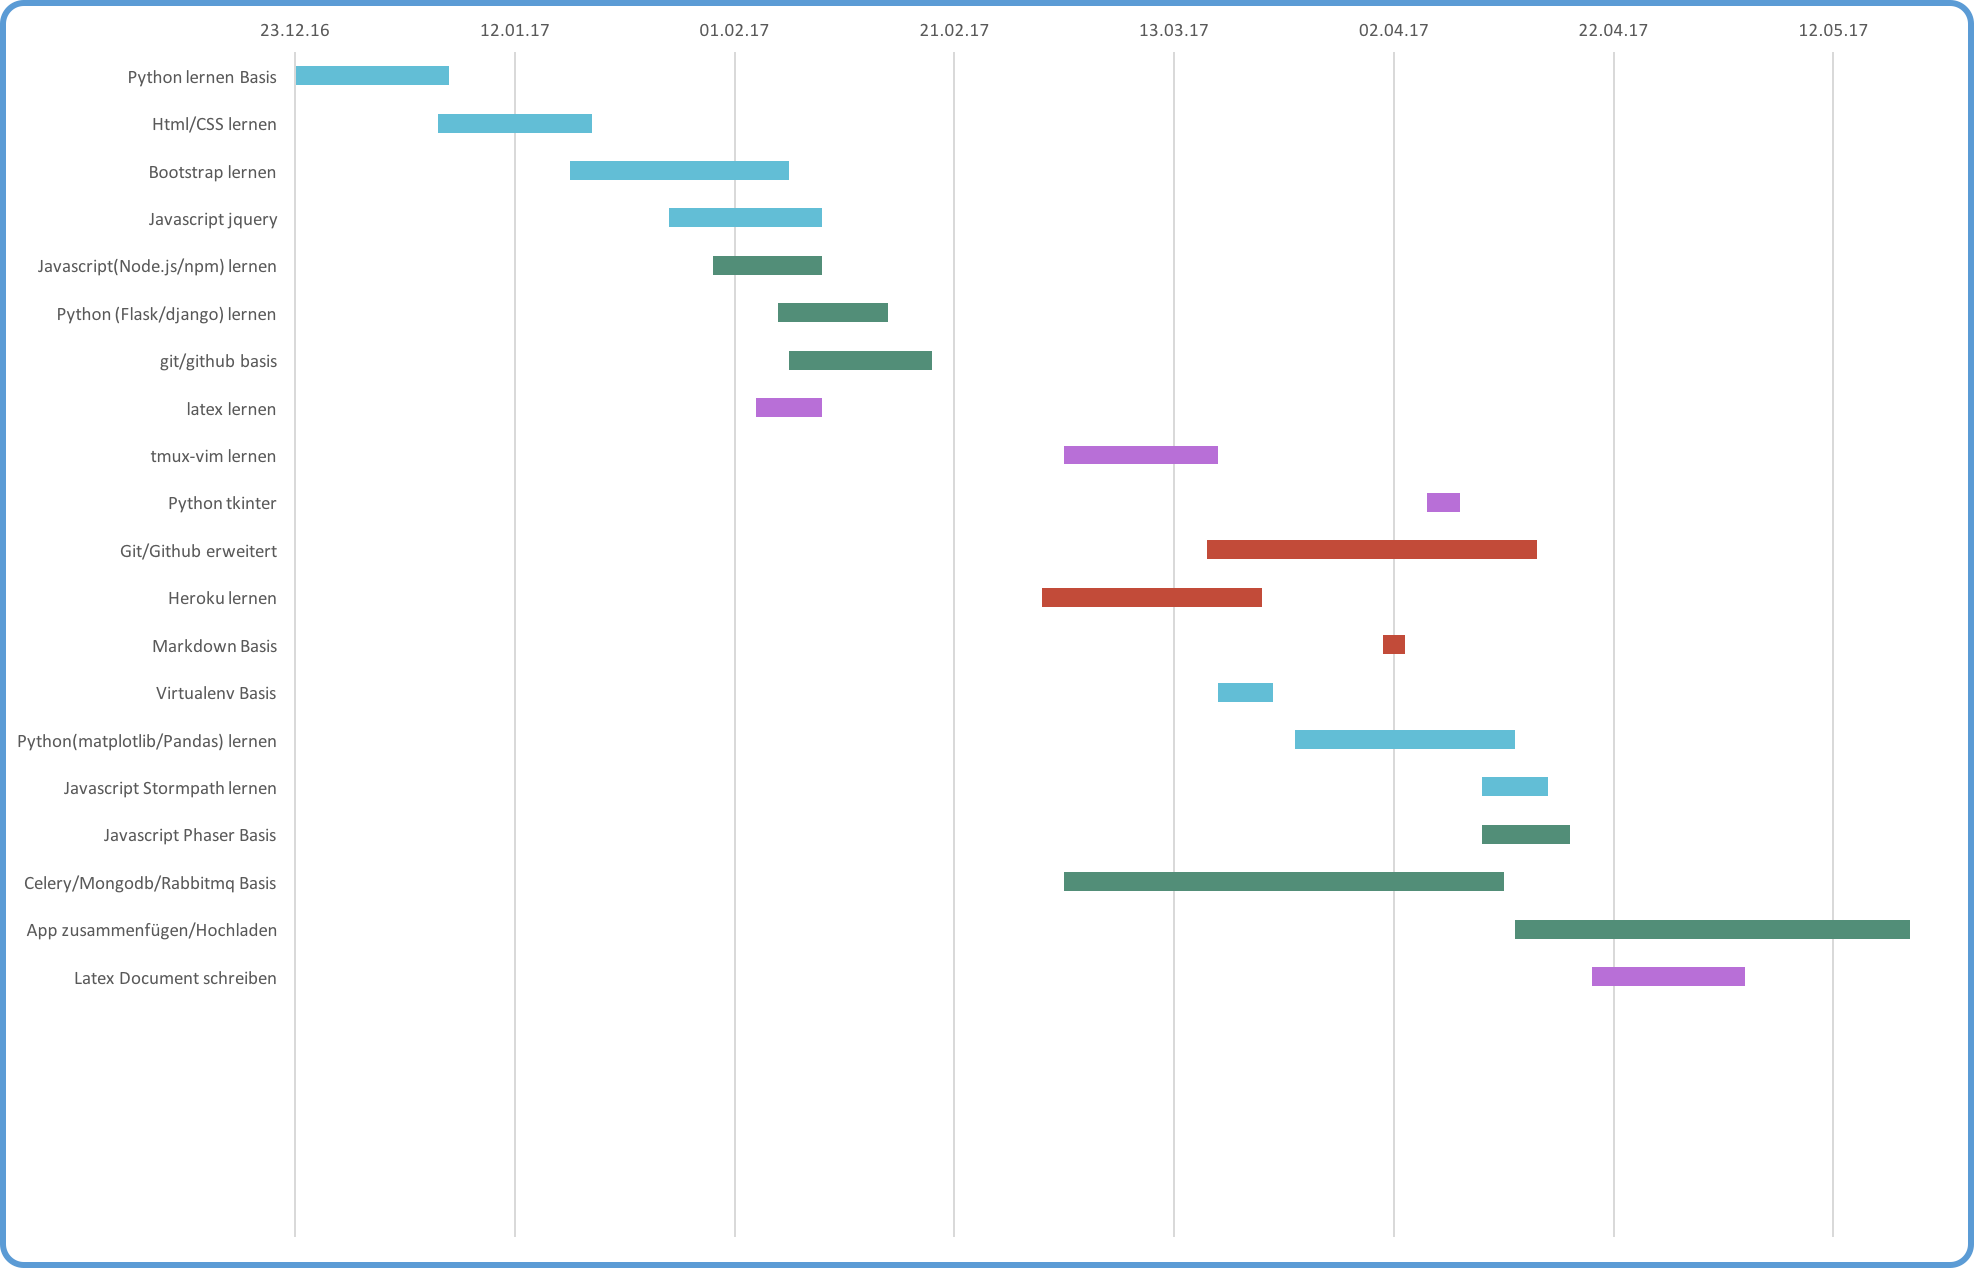
\includegraphics[width=.8\linewidth]{gantt}
%     \caption{Zeitstrahl}
%     \label{fig:sub1}
%     \end{sidewaysfigure}

\rotatebox{90}{\begin{minipage}{0.9\textheight}
\centering
    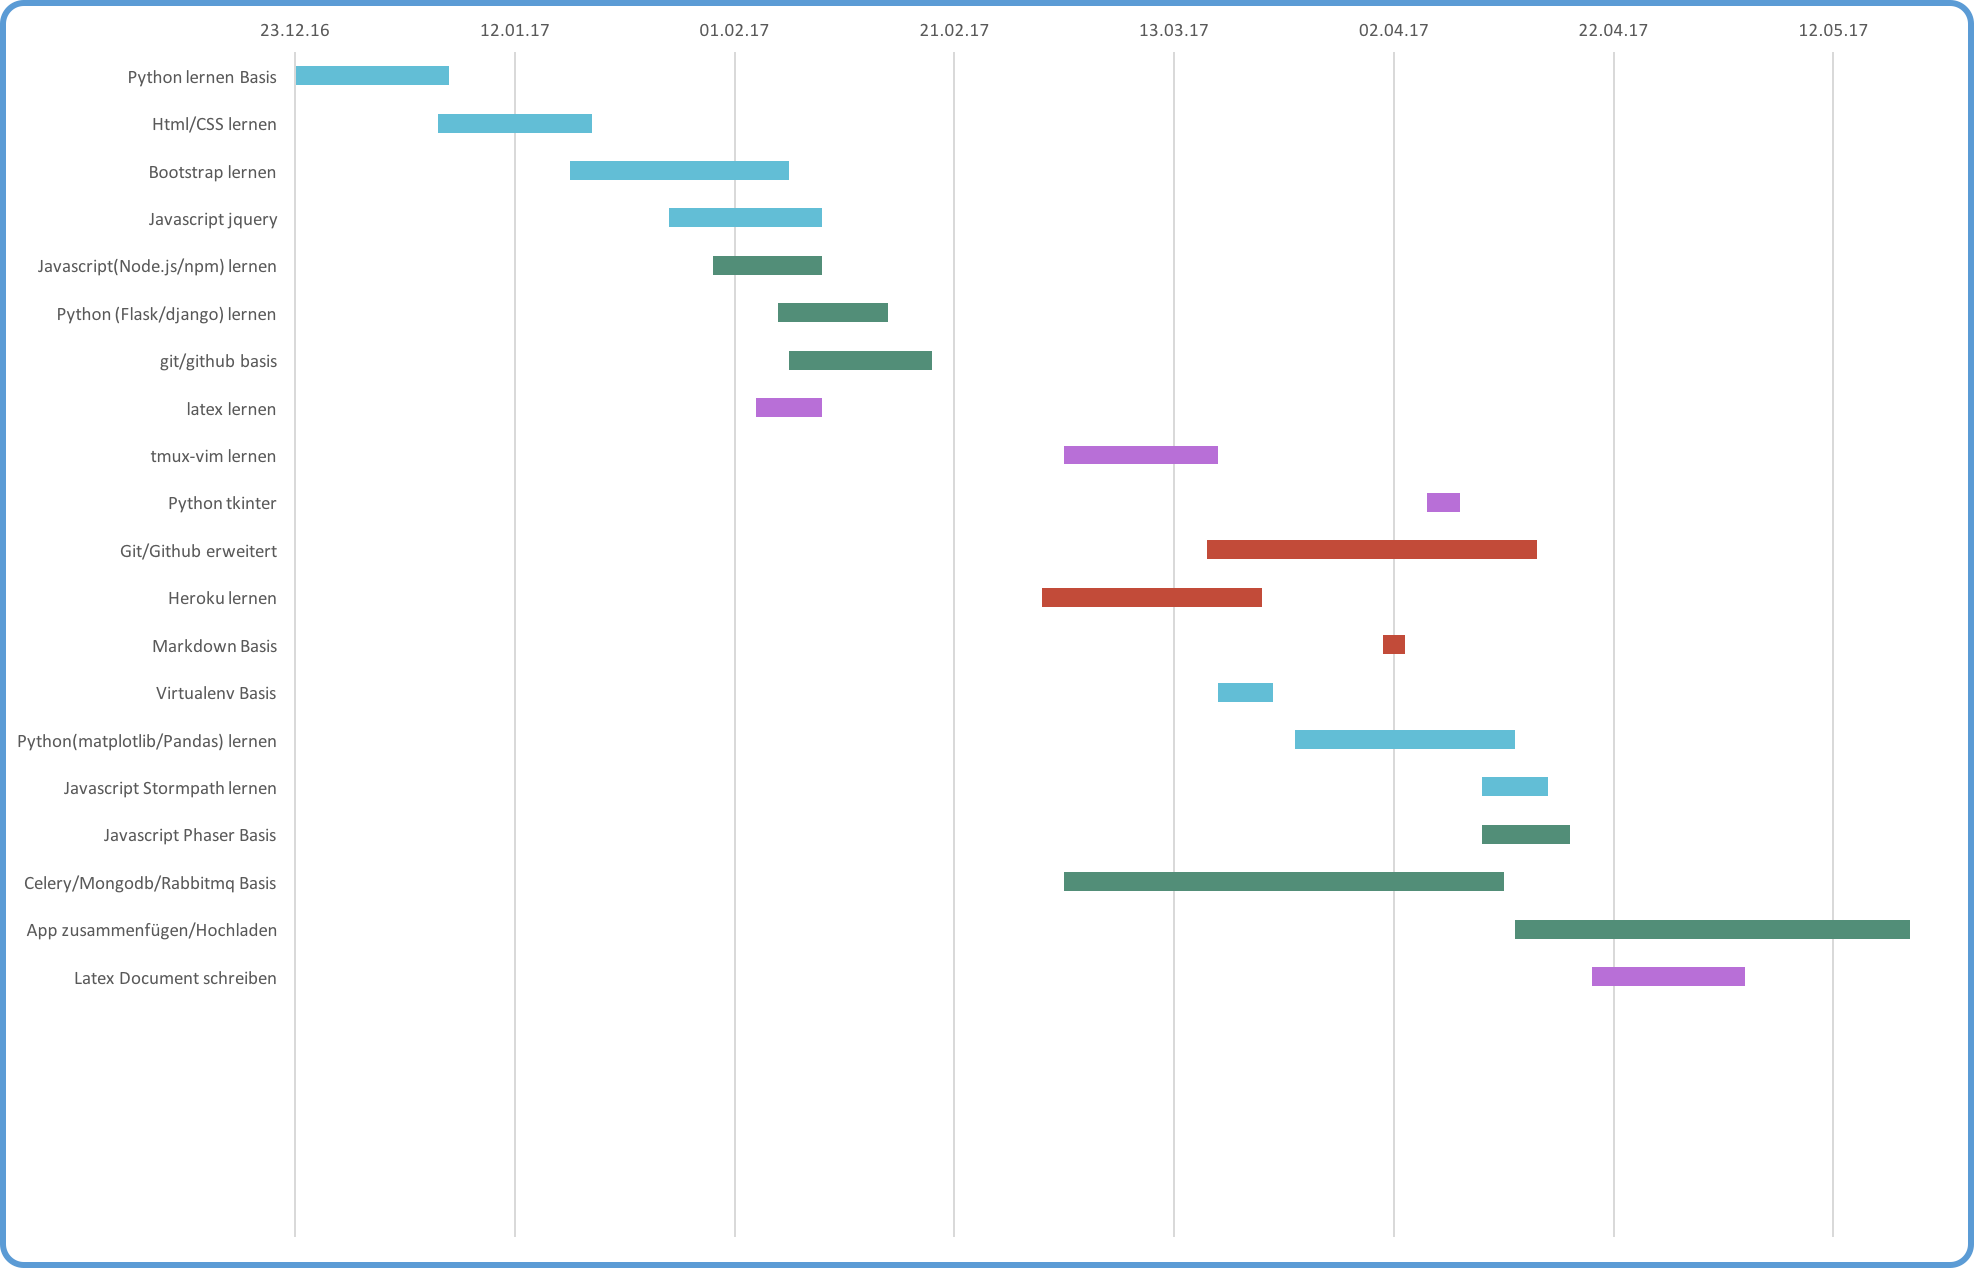
\includegraphics[width=1\textwidth]{gantt}
    \captionof{figure}{Zeitstrahl/Gantt-Tabelle}
    \label{fig:PropProf}
\end{minipage}}





\cleardoublepage


\section{Allgemeines}
In Dieser Arbeit befinden sich im Haupteil drei Einzelne Kapitel.
das Erste wird "uber die Grundlagen des Programmierens sein, wo ich zeigen werde wie und mit welchen Mitteln ich meine Webseite erstellt habe.
im Zweiten teil wird es um den Aufbau und die Struktur meiner Webseite gehen und im dritten Teil geht es um das Minigame,
welches ich mit der Engine Phaser erstellt habe.

Ich will noch betonen dass diese Arbeit sehr komplex ist und ich nat"urlich nicht in der Lage sein werde dir alles genau zu erkl"aren, da diese Arbeit ja
um die 40 Seiten umfasst. Falls du dich aber nach dem Lesen auch daf"ur interessieren solltest selber etwas zu erstellen, habe ich im Anhang noch einige Quellen
aufgelistet, welche dir helfen sollten selber durchzustarten.


\begin{figure}[ht]
    \centering
    
\includegraphics[width=.7\linewidth]{foto}
    \caption{Startbild meines Games}
    \label{fig:sub1}
    \end{figure}

\cleardoublepage












\section{html}
Hypertext Markup Language oder kurz HTML ist die Grundsprache wenn es darum geht eine Webseite zu Programmieren.
 Sie ist eine textbasierte Auszeichnungssprache zur Strukturierung digitaler Dokumente wie Texte mit Hyperlinks, Bildern und anderen Inhalten.
 HTML-Dokumente sind die Grundlage des World Wide Web und werden von Webbrowsern dargestellt.
 Neben den vom Browser angezeigten Inhalten k"onnen HTML-Dateien zus"atzliche Angaben in Form von Metainformationen enthalten, z. B.
"uber die im Text verwendeten Sprachen, den Autor oder den zusammengefassten Inhalt des Textes.
Kurz gesagt erstellt man damit die Grundstruktur der Webseite.
Oder wenn man sich die Webseite als Haus vorstellt ist HTML die W"ande und Dach/Boden.
Ein HTML document hat immer die Endung .html und man kann es direkt im Browser aufrufen ohne es vorher noch Kompilieren zu m?ssen, was sehr n"utzlich ist.
Zum Inhalt:
Ein html file besteht immer aus Head und Body und wird wie alles andere auch in Form von Tags geschrieben.
ein Beispiel <head></head> ist der head, zwischen <head> und </head> kommt der ganze Rest hinein.

Hier ein kleines Allgemeines Beispiel(Ich zeige ein allgemeines Beispiel, weil code aus meiner Website etwas komplizierter ist als "normaler html-code")

\begin{figure}[ht]
    \centering
    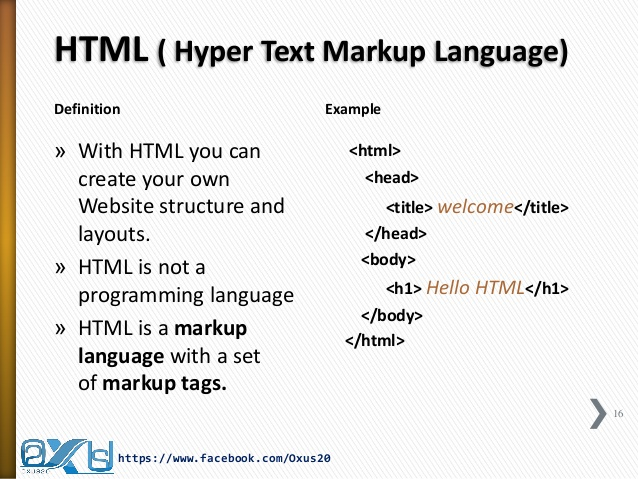
\includegraphics[width=.7\linewidth]{html-wissen}
    \caption{html-aufbau}
    \label{fig:sub1}
    \end{figure}
Zus"atzlich muss man ganz oben im head auf alle css files hinweisen, welche das html-dokument braucht z.B.:

\begin{lstlisting}
<link rel="stylesheet" href="/static/css/main.css"
\end{lstlisting}

Das gleiche f?r javascript-files, einfach im body ganz unten. z.B.:

\begin{lstlisting}
<script src="phaser.min.js"
\end{lstlisting}








\cleardoublepage


\section{css}
Cascading Style Sheets oder kurz css geh"ort wie HTMl zur Grundstruktur wenn man eine Webseite gestalten will.
Diese Sprache ist vergleichbar mit Farbe, denn mit ihr will man die Seite sch"oner und attraktiver Gestalten.
css ist ein "living standard", das heisst sie wird st"andig weiterentwickelt.
Bei css benutzt man nicht wie bei html tags wie <head></head> sondern es sieht in etwa so aus:\\
\begin{lstlisting}
  body {
    font-size: 1em;
    color: #777B7E;
    font-weight: 400;
    background: #D3D8DC;
    position: relative;
  }
\end{lstlisting}







Mit css arbeitet man so:\\
man w"ahlt den Oberbegriff aus dem Html-File (hier body)\\
dann setzt man in Klammern ({}) was ver"andert werden soll.\\
man kann w"ahlen zwischen vielen Sachen wie z.B. der H"ohe oder der Breite.\\
Nat?rlich muss man im html-File angeben, dass man dieses css-File benutzt um
ver"anderungen and der Struktur der Seite vorzunehmen.\\
Diese Referenz sieht dann wie folgt aus:


\begin{lstlisting}
<link rel="stylesheet" href="/static/css/main.css"
\end{lstlisting}


\begin{figure}[ht]
    \centering
    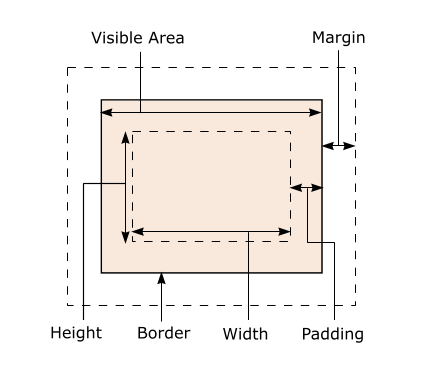
\includegraphics[width=.7\linewidth]{css-box}
    \caption{css aufbau}
    \label{fig:sub1}{Hier wird veranschaulicht wie man die Form ver"andern kann.}
    \end{figure}

\cleardoublepage


\section{jquery}






Jquery ist ein Framework welches auf Javascript basiert.
Jquery wird benutzt um animationen und andere Funktionen in die Webseite hineinzubringen.
Ich benutze einige Jquery-Plugins welche ich von der Webseite jqueryrain herhabe.
Von dieser Seite hole ich mir die Komplexen Codebl"ocke, welche ich noch in mein eigenes Framework einf?gen muss.
ich muss sie noch ver"andern damit sie genau in meine Webseite hineinpasst.
Hier ein paar Beispiele:









\section{meine jquery-Plugins}

\begin{figure}[ht]
    \centering
    
\includegraphics[width=.6\linewidth]{sticky}
    \caption{Sticky}
    \label{fig:sub1}{mit sticky kann ich den Titel befestigen wenn ich runterscrolle,d.h. er kommt mit runter.}
    \end{figure}

    \begin{figure}[ht]
        \centering
        
\includegraphics[width=.6\linewidth]{carousel}
        \caption{carousel}
        \label{fig:sub1}{mit dem Karussel kann ich auf interessante zwischen Bilder switchen.}
        \end{figure}

        \begin{figure}[ht]
            \centering
            
\includegraphics[width=.6\linewidth]{gallery}
            \caption{gallery}
            \label{fig:sub1}{mit der Gallery sieht man zuerst alle Bilder verkleinert und wenn man draufklickt vergr?ssern sie sich.}
            \end{figure}

            % \begin{figure}[ht]
            %     \centering
            %     
\includegraphics[width=.5\linewidth]{paint}
            %     \caption{Javascript und jquery logo}
            %     \label{fig:sub1}
            %     \end{figure}
            %
            %     \begin{figure}[ht]
            %         \centering
            %         
\includegraphics[width=.5\linewidth]{background}
            %         \caption{Javascript und jquery logo}
            %         \label{fig:sub1}
            %         \end{figure}
            %
            %         \begin{figure}[ht]
            %             \centering
            %             
\includegraphics[width=.7\linewidth]{modernizr}
            %             \caption{Javascript und jquery logo}
            %             \label{fig:sub1}
            %             \end{figure}








\cleardoublepage



\section{Flask}


\subsection{Python-allgemein}

Python ist eine Interpretierte, object-orientierte programmiersprache mit dynamischer Semantic.
Python is einfach zu lernen im Vergleich zu C oder Java und sie ist auch sehr einfach zu lesen.
Programmierer suchen sich auch oft diese Programmiersprache aus, weil man Fehler einfach finden kann man sich dadurch viel Wartung erspart.
\subsection{flask-allgemein}

Flask ist ein in Python geschriebenes Webframework. Der Fokus von Flask liegt auf Erweiterbarkeit und guter Dokumentation.
Die einzigen Abh"angigkeiten sind Jinja2,
eine Template Engine, und Werkzeug, eine Bibliothek zum Erstellen von WSGI-Anwendungen.
WSGI heisst Web Server Gateway Interface, d.h. es stellt dir einen Server zur Verf"ugung
% \subsection{flask-vereinfacht}
% Flask ist wie der Backend Router der zeigt wo welche seite erscheint und mir viele Werkzeuge zur Verf"ugung stellt.
% Um Flask laufen zu lassen, muss ich nur python app.py im richtigen Ordner im Terminal eingeben, wobei app.py das File ist
% z.B: kann ich meine Flask-Webseite lokal im Browser auf Pfad 8080 laufen lassen, wenn ich im terminal eingebe
% cd idpa
% python app.py
% und sehe bei der URL-Pfad:
% dass es die Index seite geladen hat, wie ich es im Python-router-file programmiert habe.


Die Minimalanforderungen von Flask sind folgende:
\begin{lstlisting}
  from flask import Flask
  app = Flask(__name__)

  @app.route("/")
  def hello():
      return "Hello World!"

  if __name__ == "__main__":
      app.run()
\end{lstlisting}
wenn man dann im Terminal eingibt:

\begin{figure}[ht]
    \centering
    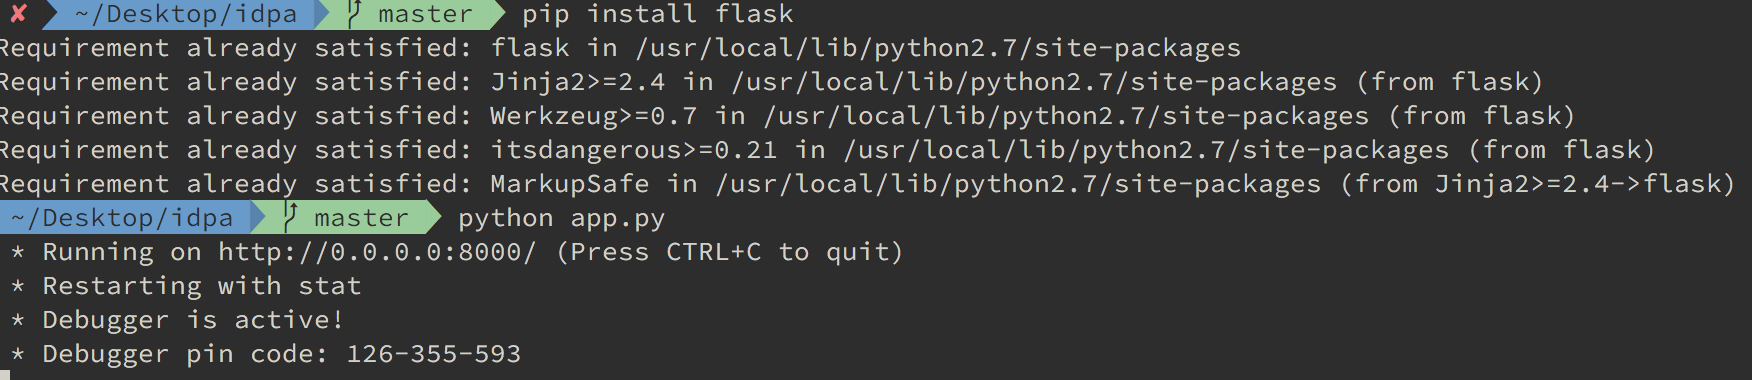
\includegraphics[width=1\linewidth]{python-app}
    \caption{Flask-App starten}
    \label{fig:sub1}
    \end{figure}

    Sieht man dass man auf Port 8000 seine Webseite lokal "offnen und anschauen kann.
    Man muss im Browser nur 0.0.0.0:8000 eingeben dann gelangt man zu seiner Seite.

    \cleardoublepage

% von Flask importiere ich alles n"otigen Bibliotheken um mein Project z.B:\\
% Sicherer zu machen beim Login. Dies mithilfe von der Bibliothek:
% \begin{lstlisting}
% from flask_bcrypt import generate_password_hash
% \end{lstlisting}
% welches ich im File models.py eingef?gt habe.
% Dies erlaubt es mir
%
\section{phaser Engine}
Phaser ist eine game-Engine welche als Basis (mit eingebauter Physik und anderer Logik) daf"ur dient, sein eigenes Spiel darauf zu erstellen.
Phaser ist eine gute Gameengine welche f"ur Anf"anger geeignet ist, ich zum Beispiel habe in wenigen Wochen ein eigenes Minispiel kreieren k"onnen mit
relativ kleinem Aufwand.\\
Mit eingebauter Physik meine ich das man Figuren in sein eigenes Game einbetten kann, welche an Physikalische Gesetze gebunden sind.
das heisst ich kann einen Stein in mein Game einbinden und ihn dann so programmieren, dass er z.B. immer herunterf"allt, wenn ihn der Spieler anst"osst.
\begin{figure}[ht]
\centering
\begin{subfigure}{.5\textwidth}
  \centering
  
\includegraphics[width=.5\linewidth]{phaser}
  \caption{gitlogo}
  \label{fig:sub1}
\end{subfigure}%
\begin{subfigure}{.5\textwidth}
  \centering
  
\includegraphics[width=.5\linewidth]{foto}
  \caption{Githublogo}
  \label{fig:sub2}
\end{subfigure}
% \caption{}
% \label{fig:test}
% \caption[short title]{}
\end{figure}




\cleardoublepage

\section{Datenbanken}
Die Programmiersprache mit welcher man Datenbanken programmieren kann heisst. sql oder sequel:
Datenbanken werden gebraucht um Daten darin zu speichern, es gibt viele verschiedene Arten, ich habe mich f?r sqlite entschieden, weil sie eher eine einfache version ist und vor allem f?r Anf?nger gedacht ist.
Ich habe also die Datenbank genannt sqlite mithilfe der Pythonbibliothek genannt Peewee erstellt.
Dank Peewee musste ich nicht auch noch die Programmiersprache sql lernen, bei der es um Datenbanken geht, denn Peewee erstellt mir einfach eine.



\begin{figure}[ht]
    \centering
    
\includegraphics[width=.5\linewidth]{database}
    \caption{Logo Databases}
    \label{fig:sub1}{Wie sie sehen gibt es verschiedene Arten von Datenbanken.}
    \end{figure}

    \begin{figure}[ht]
        \centering
        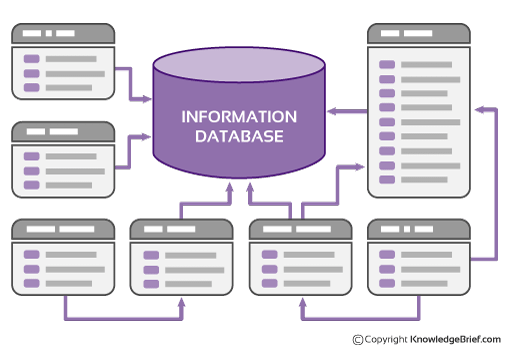
\includegraphics[width=.8\linewidth]{database1}
        \caption{Logo Databases}
        \label{fig:sub1}{}
        \end{figure}
% Nun zu meinem project:\\
% in meinem Project habe ich ein File welches models.py heisst, darin steht:
%
%
%
%     \begin{lstlisting}
%       from peewee import *
%       DATABASE = SqliteDatabase('social.db')
%     \end{lstlisting}
%     Hier f?ge ich die Datenbank sqlite mithilfe von peewee ein.\\
%
%   weiter unten im selben File kann man sehen:
%     \begin{lstlisting}
%     def initialize():
%     DATABASE.connect()
%     DATABASE.create_tables([User, Post, Relationship], safe=True)
%     DATABASE.close()
%     \end{lstlisting}
%

\cleardoublepage































\section{Text Editor}

Programmieren tut man nicht mit Word oder Excel oder Powerpoint.
Man braucht einen anst"andigen Text Editor,
welcher mit wichtigen Sachen wie zum Beispiel syntax highlighting ausgestattet ist, damit man seinen Code besser betrachten kann.
Zudem kann ein Text Editor vieles was man eigentlich im Terminal tun m"usste, und kann es sogar leichter und schneller machen.
Jeder Anf"anger im Programmieren weiss, dass man einen Text Editor braucht gut Programmieren zu k"onnen.
Die Frage ist nur (und das besch?ftigt auch fortgeschrittene Programmierer) welcher man verwenden sollte.
Ich habe Meine Webseite im Text Editor Atom und das Game in Brackets programmiert.
Atom weil es feature-reich ist und brackets wegen der Livevorschau, welche es mir erm?glicht ver?nderungen von meinem Game Live anzusehen.
\begin{figure}[ht]
    \centering
    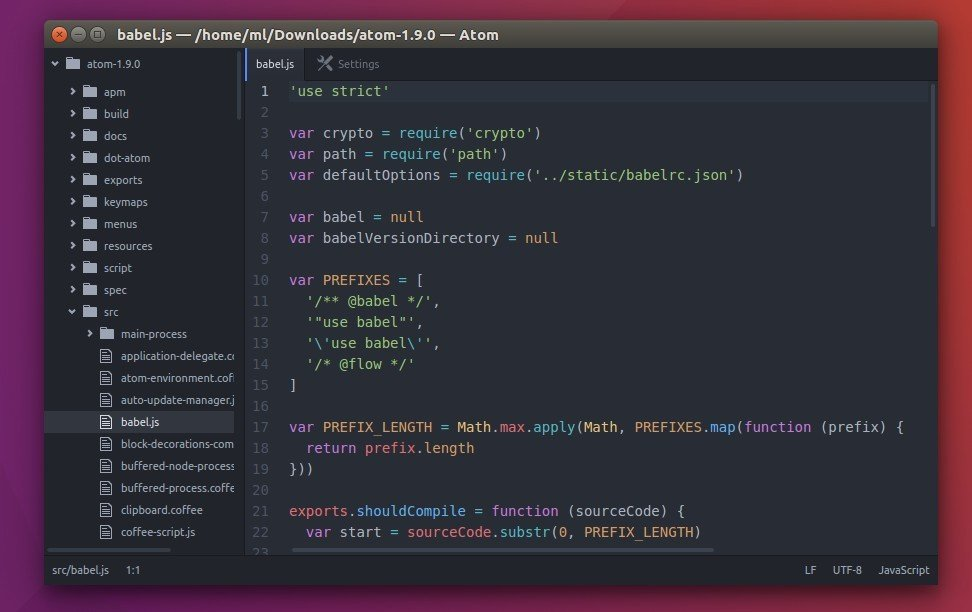
\includegraphics[width=.6\linewidth]{text-editor}
    \caption{Beispiel Terminal}
    \label{fig:sub1}{Hier sehen sie den Text Editor Atom.\\
    Links befindet sich die Auflistung aller Files und Ordner\\
    Rechts ist der Platz wo man Code schreibt}
    \end{figure}




    \begin{figure}[ht]
        \centering
        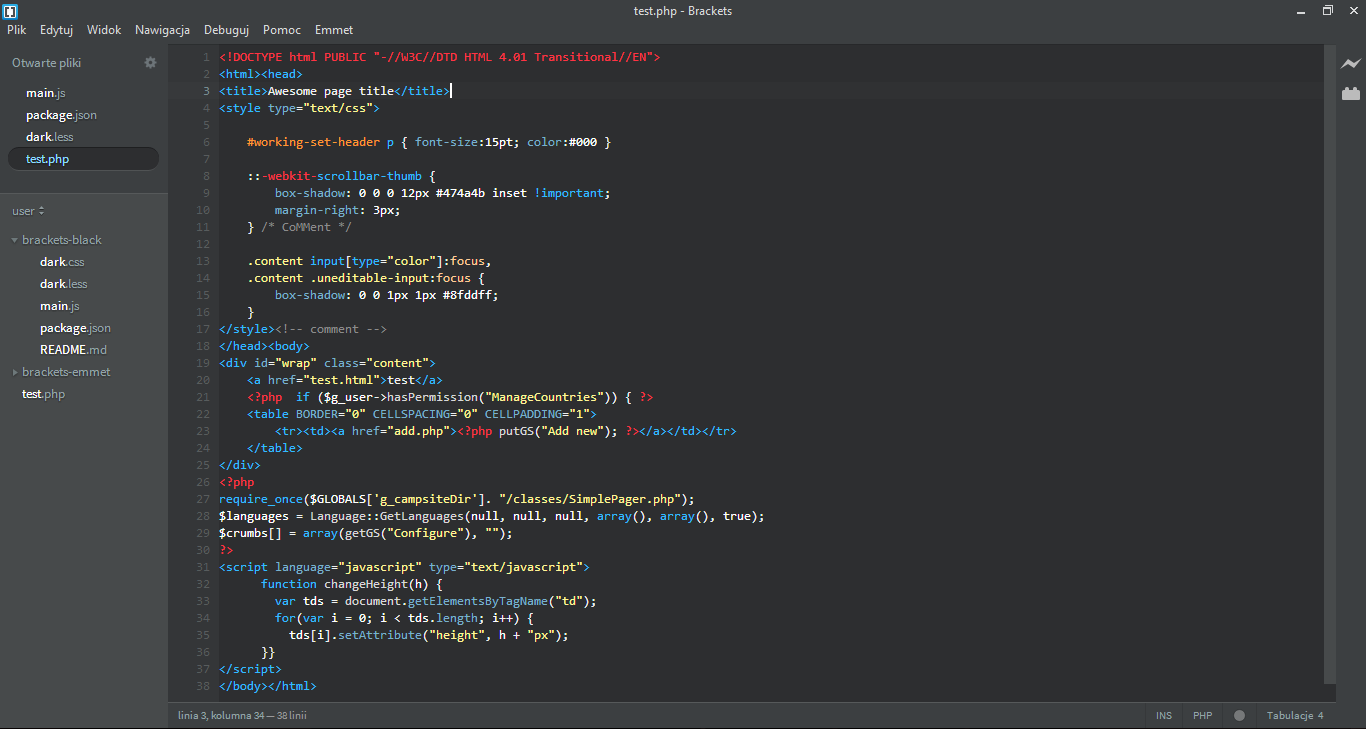
\includegraphics[width=.6\linewidth]{brackets}
        \caption{Beispiel Terminal}
        \label{fig:sub1}{Brackets ist "ahnlich wie Atom aufgebaut.\\
        Zu beachten ist rechts oben der LiveVorschau-knopf.}
        \end{figure}

\cleardoublepage












\section{Git und Github}
Git ist ein freies und open source Kontrollsystem um alles von kleinen zu gr"osseren
Projecten zu handeln.
Git ist einfach zu lernen und hat zugleich eine mega schnelle Verarbeitungsgeschwindigkeit
Es ist besser als manch andere SCM (bla bal) tools wie etwa Subversion, CVS, Perforce
und ClearCase.
Mit Features wie etwa einfaches teilen seiner arbeiten, bequemes staging und multiple Workflows.
\begin{figure}[ht]
\centering
\begin{subfigure}{.5\textwidth}
  \centering
  
\includegraphics[width=.5\linewidth]{git_logo}
  \caption{gitlogo}
  \label{fig:sub1}
\end{subfigure}%
\begin{subfigure}{.5\textwidth}
  \centering
  
\includegraphics[width=.5\linewidth]{github}
  \caption{Githublogo}
  \label{fig:sub2}
\end{subfigure}
% \caption{}
% \label{fig:test}
% \caption[short title]{}
\end{figure}

\begin{figure}[ht]
    \centering
    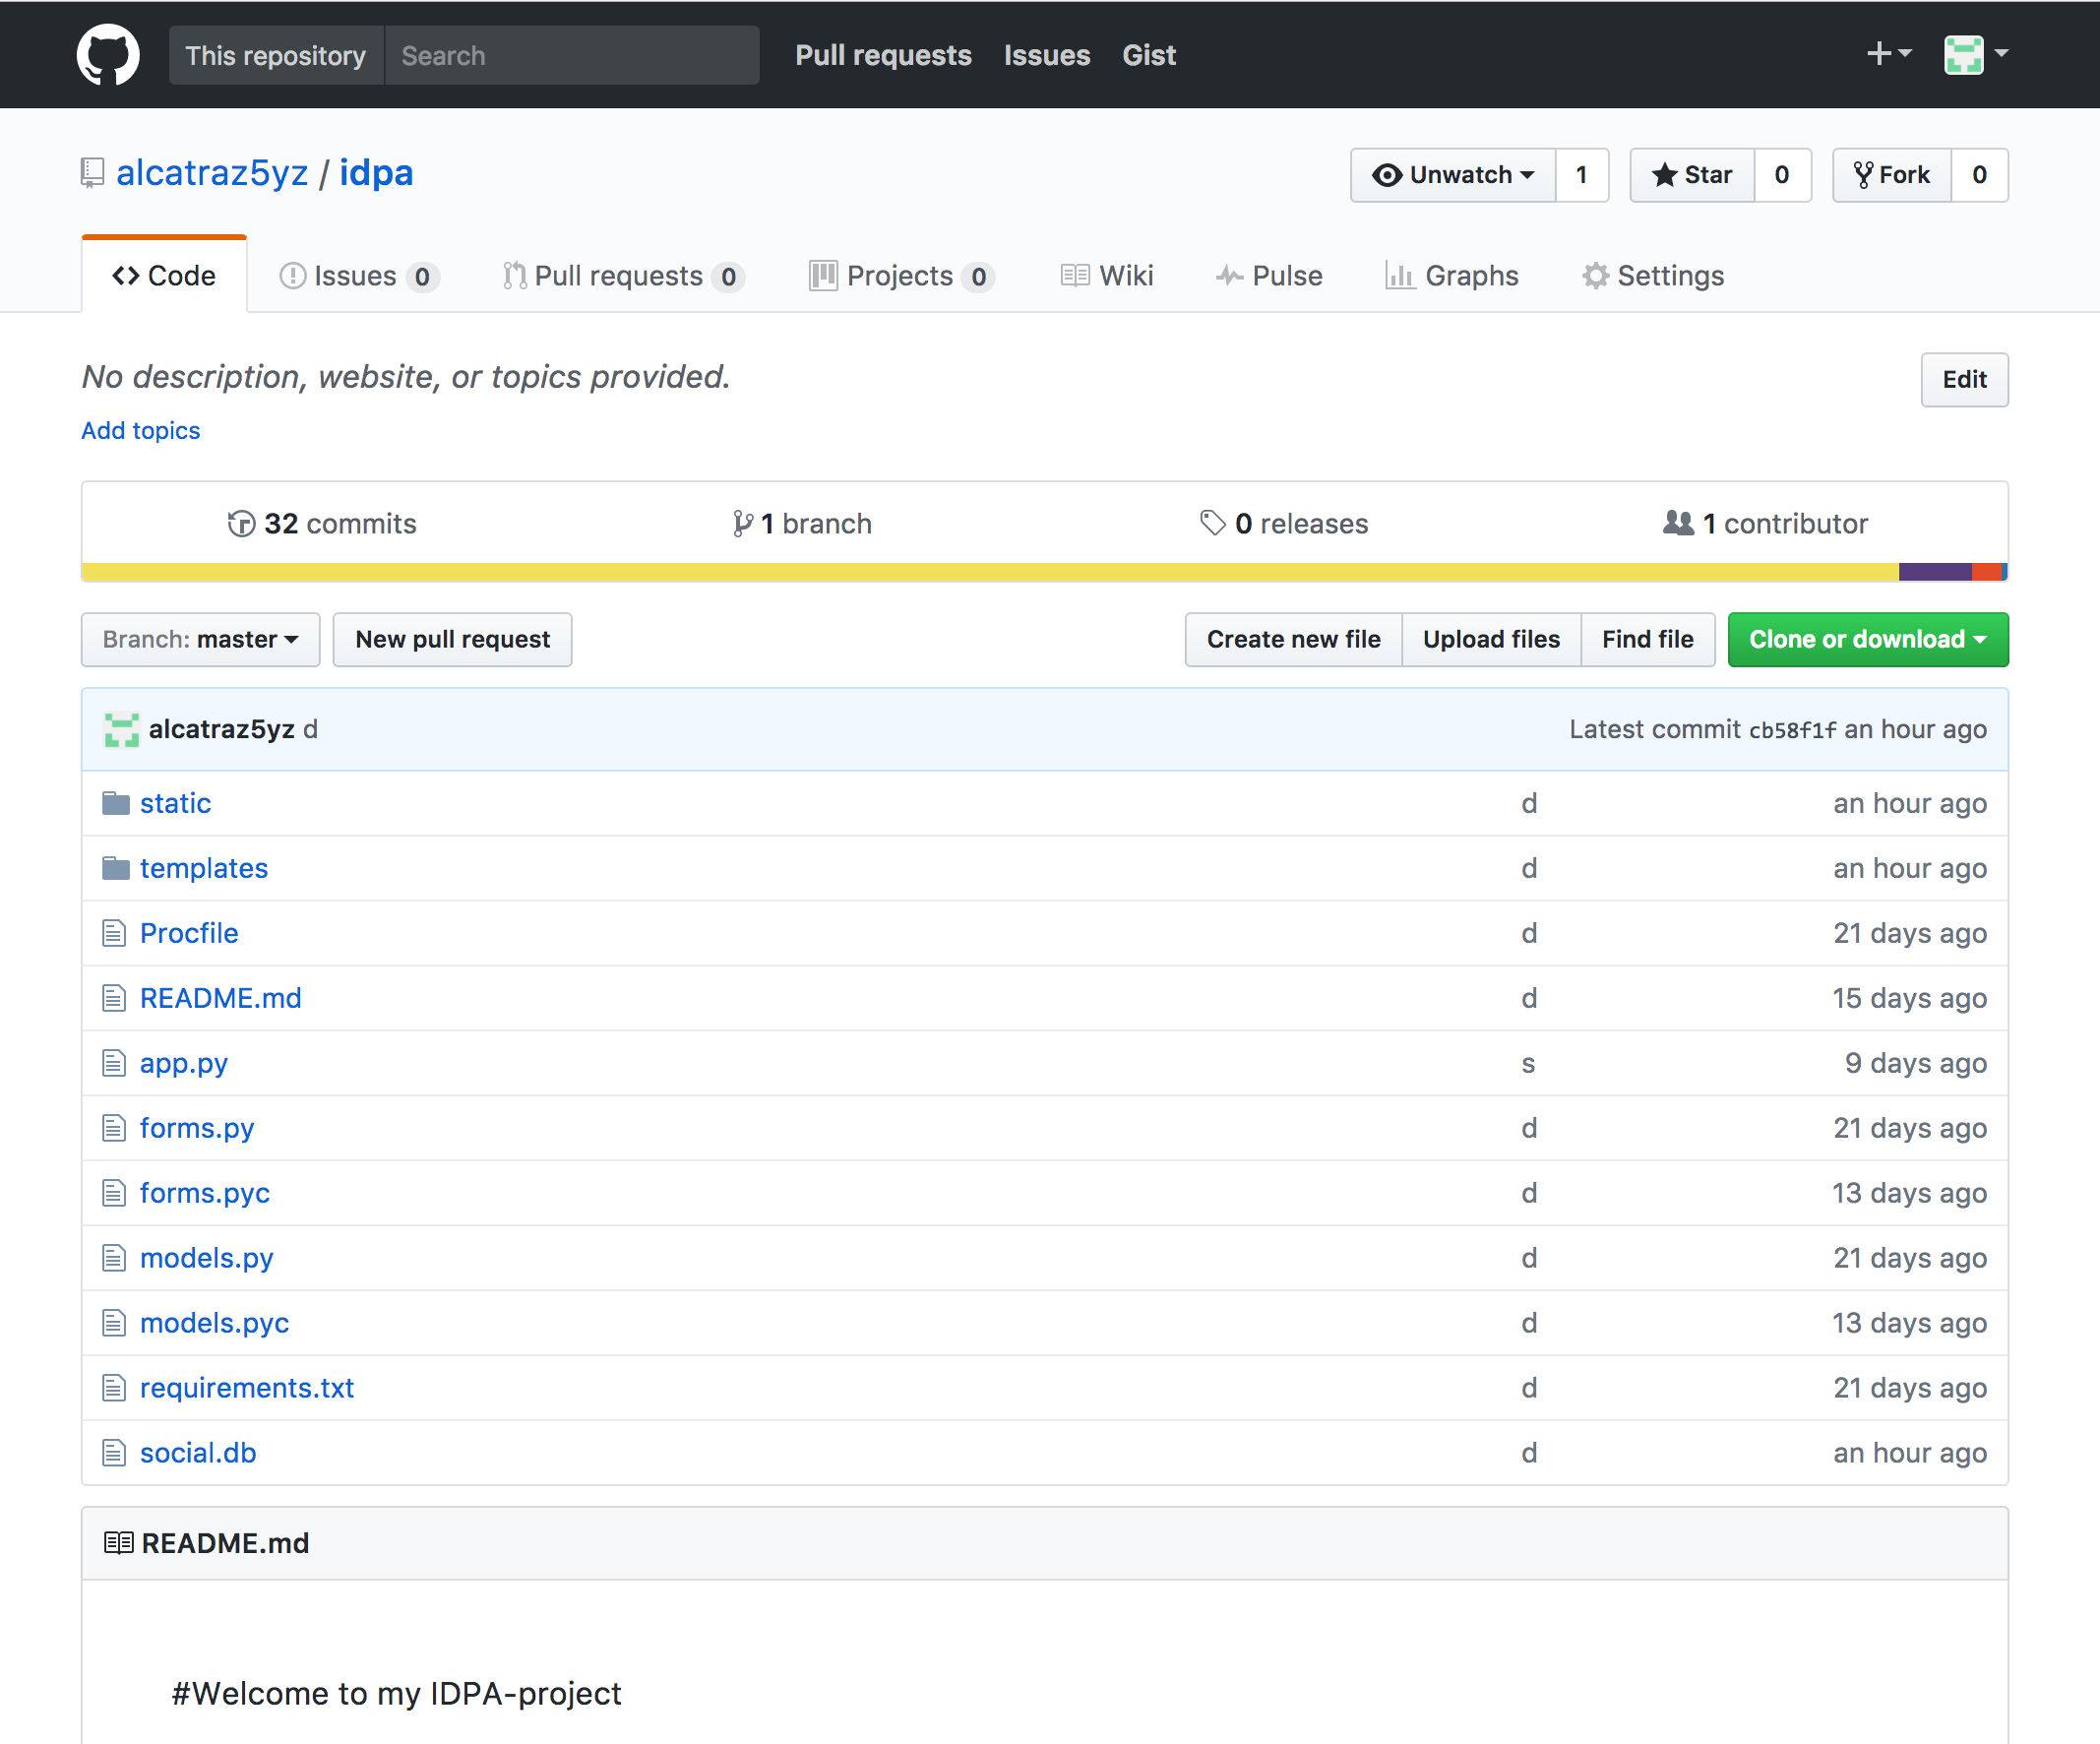
\includegraphics[width=.7\linewidth]{github-repo}
    \caption{Github}
    \label{fig:sub1}{Hier sieht man mein Github Repository, d.h. mein ganzer Code ist hier dargestellt.
    Man sieht oben auch noch dass man viele Optionen hat Ver?nderungen vorzunehmen}
    \end{figure}

    % \begin{figure}[ht]
    %     \centering
    %     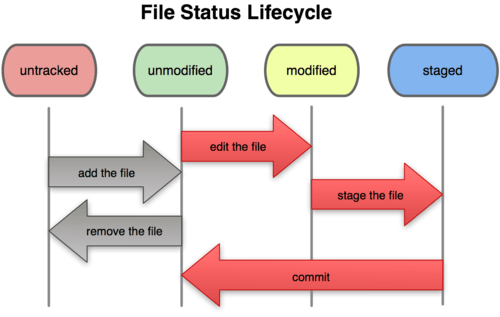
\includegraphics[width=.7\linewidth]{git}
    %     \caption{Hier sieht }
    %     \label{fig:sub1}
    %     \end{figure}

\cleardoublepage











% \section{Bower}
% Bower ist ein netter kleiner Helfer, der es mir Erm?glicht Plugins z.B. von Jquery bequem von meinem Terminal in mein Project einzubinden, ohne auf die
% jeweilige Webseite gehen zu m?ssen und den Code da zu suchen.
%
%
% \begin{figure}[ht]
%     \centering
%     
\includegraphics[width=.5\linewidth]{bower}
%     \caption{Version control}
%     \label{fig:sub1}
%     \end{figure}
%
% \cleardoublepage















\section{Latex}
Latex ist eine Programmiersprache, welche es mir erm"oglicht dokumente wie mit Word zu schreiben.
Mit Latex muss man die Einstellungen selber Programmieren, was man mit Word nicht muss.
Bei Word ist das so, dass man zwar nicht selber programmieren muss, daf"ur muss man aber den richtigen Abschnitt mit dem Richtigen Knopf finden.
Wenn man also ein schneller Typer ist und die Befehle auswendig kann, ist man viel schneller mit Latex als mit Word, weil man nicht erst noch die Kn"opfe suchen muss.
Zus"atzlich kann man mit Latex Mathematische Formeln viel einfacher auflisten und darstellen.
Da man mit Latex alles selber programmieren muss, kann man auch genau sagen wo welcher Text hin soll.
Dad heisst kein h"assliches Verschieben des Textes mehr wie in Word.

Aufbau: Das Latex-File ist wie ein html-File aufgebaut, das heisst es besteht aus "head" welcher die Pakete beinhaltet welche man braucht und aus "body"
welcher die Oberfl?che darstellt, welche man ansehen kann.
Falls du es nocht nicht gemerkt hast, dieses Dokument wurde ebenfalls mit Latex erstellt.


\begin{figure}[ht]
    \centering
    
\includegraphics[width=.6\linewidth]{latex-plakat}
    \caption{Latex-Plakat}
    \label{fig:sub1}{Hier sieht man aus was ein Latex-File alles besteht, n?mlich aus Head mit den Importierten Packages und
    dem Body mit dem text.}
    \end{figure}

\cleardoublepage
















\section{heroku}
Heroku ist ein Cloud dienst welcher es mir erm"oglicht meine Flask-Webseite hochzuladen.
Heroku ist auf einige Sprachen und Frameworks besonders gut ausger"ustet, welches es erleichtert sie Hochzuladen falls es irgendwelche ausnahmen gibt.
Heroku ist gratis bis zu einem bestimmten Punkt, das heisst man kann bis zu 5 Webseiten gratis hochladen.
die Downsite ist, dass die hochgeladene Seite die URL z.B. www.Beispiel.herokuapp.com hat. (Siehe herokuapp ist darin enthalten.)

F"ur Programmierer ist es sehr bequem ihre Seite auf Heroku zu laden, denn man kann sie einfach in dem Terminal hochladen und muss nicht extra auf die Seite
von Heroku gehen und sie dort hochladen, es geht aber nat"urlich auch.


\begin{figure}[ht]
    \centering
    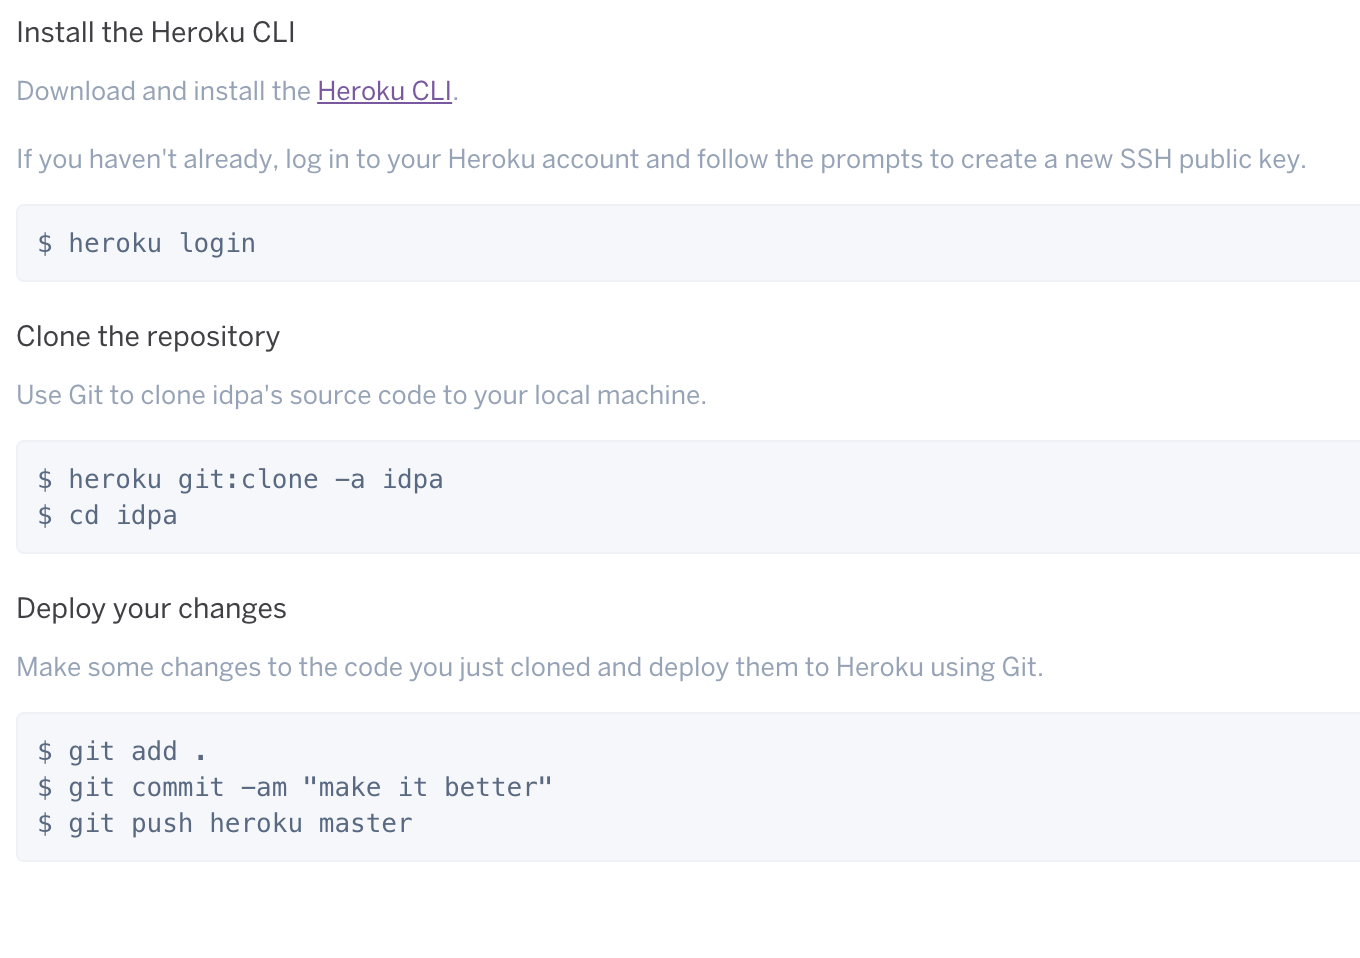
\includegraphics[width=.6\linewidth]{heroku-instructions}
    \caption{Dies ist ein Bild von der Heroku webseite:\\
    man sieht es hat dort eine gute erkl"arung wie man alles Handeln kann.}
    \label{fig:sub1}
    \end{figure}

    \begin{figure}[ht]
        \centering
        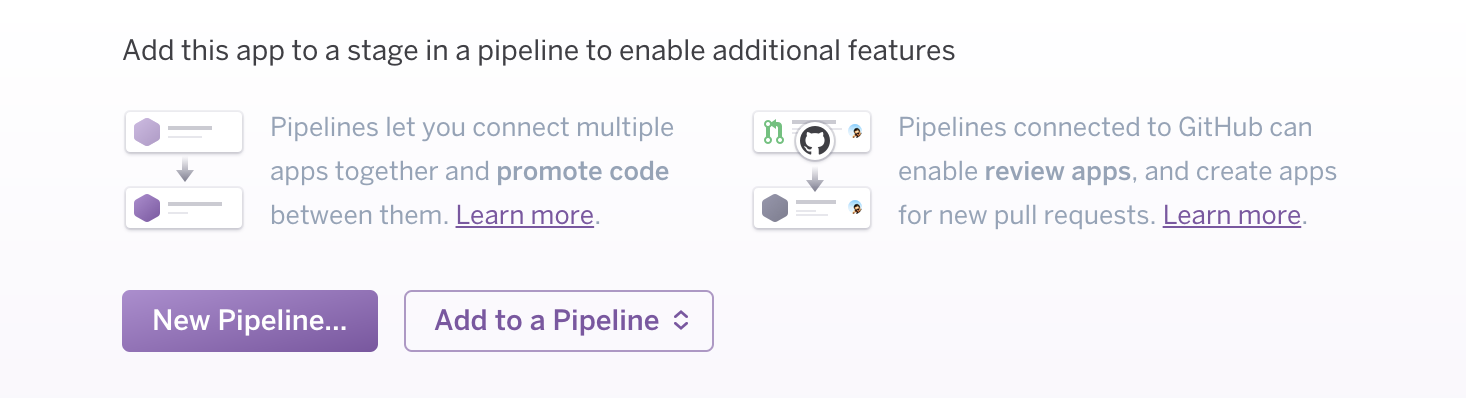
\includegraphics[width=.7\linewidth]{heroku-pipeline}
        \caption{Es gibt auch zus"atzliche Features}
        \label{fig:sub1}
        \end{figure}




\begin{figure}[ht]
    \centering
    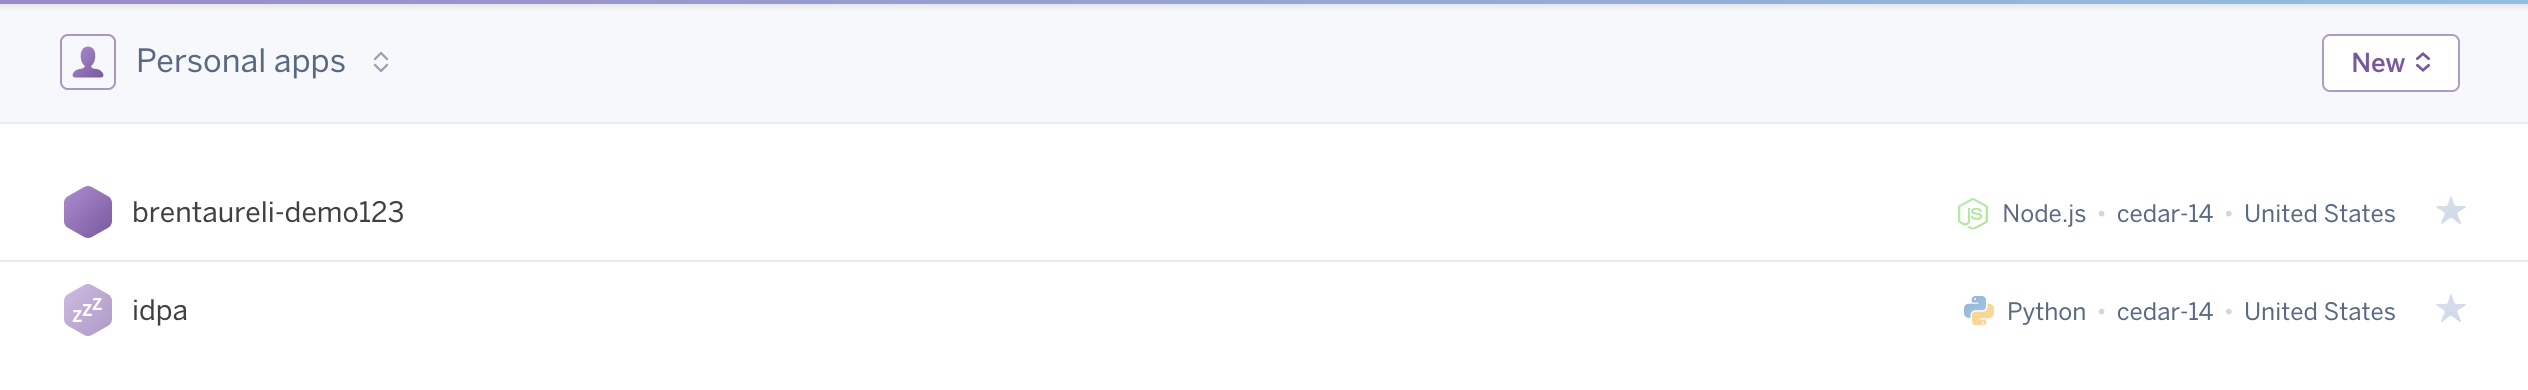
\includegraphics[width=.8\linewidth]{heroku-apps}
    \caption{Hier sieht man meine Apps welche ich auf Heroku hochgeladen habe, das einte ist meine idpa}
    \label{fig:sub1}
    \end{figure}
\cleardoublepage






\section{CLI/Terminal/cmd/Powershell/iTerm}


\begin{figure}[ht]
\centering
\begin{subfigure}{.5\textwidth}
  \centering
  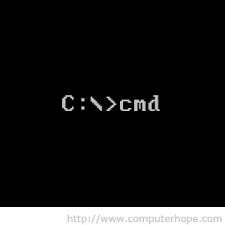
\includegraphics[width=.5\linewidth]{download-1}
  \caption{logo cmd}
  \label{fig:sub1}
\end{subfigure}%
\begin{subfigure}{.5\textwidth}
  \centering
  
\includegraphics[width=.5\linewidth]{download-2}
  \caption{allgemeines Logo}
  \label{fig:sub2}
\end{subfigure}
% \caption{}
% \label{fig:test}
% \caption[short title]{}
\end{figure}


Eines der vermutlich wichtigsten Tools ist wohl der Terminal unter Windows Usern auch als CMD bekannt.
Mit dem Terminal kann man so ziemlich alles machen.\\
man kann sogar zwei arten von Text Editoren im Terminal laufen lassen(vim und nano).
Ich mache meine Arbeit aber mit Atom und Brackets.\\
\subsection{Wof"ur ich den Terminal f"ur meine Arbeit alles brauche}

Ich benutze den Terminal f"ur vielerlei:\\
1. um Meine erstellte Webseite Lokal laufen zu lassen und zu schauen ob sie geht\\
2. um meinen Code auf Github zu laden und zu holen wenn n"otig,das heisst mein Code verwalten.\\
3. um meinen Code auf Heroku zu laden\\
4. um allgemeines zeugs zu tun wie etwa neues file/Ordner erstellen\\



\begin{figure}[ht]
    \centering
    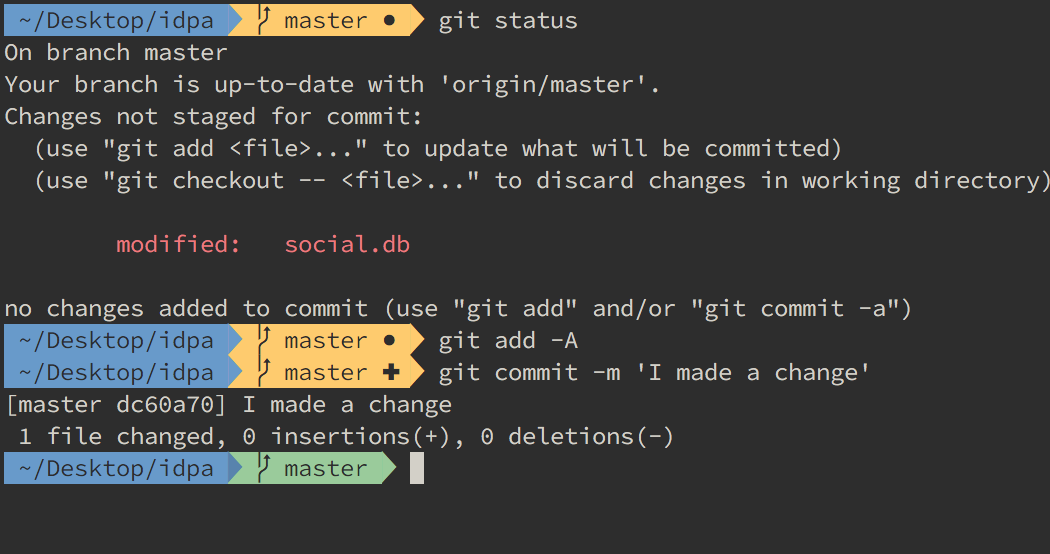
\includegraphics[width=.7\linewidth]{cli}
    \caption{Beispiel Terminal}
    \label{fig:sub1}{Hier sehen sie mein Terminal,(
    ich benutze iTerm auf meinem Macbook Pro),
    worin ich gerade
    die Version von meinem Project mithilfe von Git aktualisiere.}
    \end{figure}

    \cleardoublepage

    \begin{figure}[ht]
        \centering
        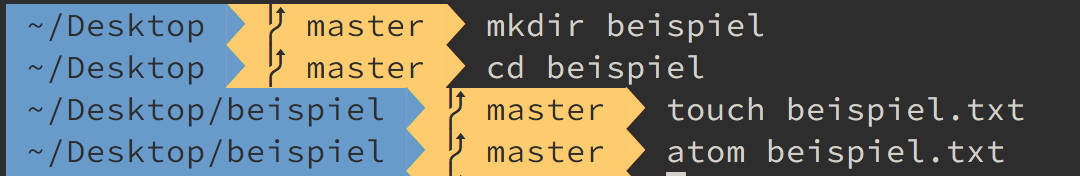
\includegraphics[width=.7\linewidth]{cli-einfaches}
        \caption{Beispiel Terminal}
        \label{fig:sub1}{Einfaches Kreieren der Files und Ordner geh"ort auch dazu.}
        \end{figure}


        \begin{figure}[ht]
            \centering
            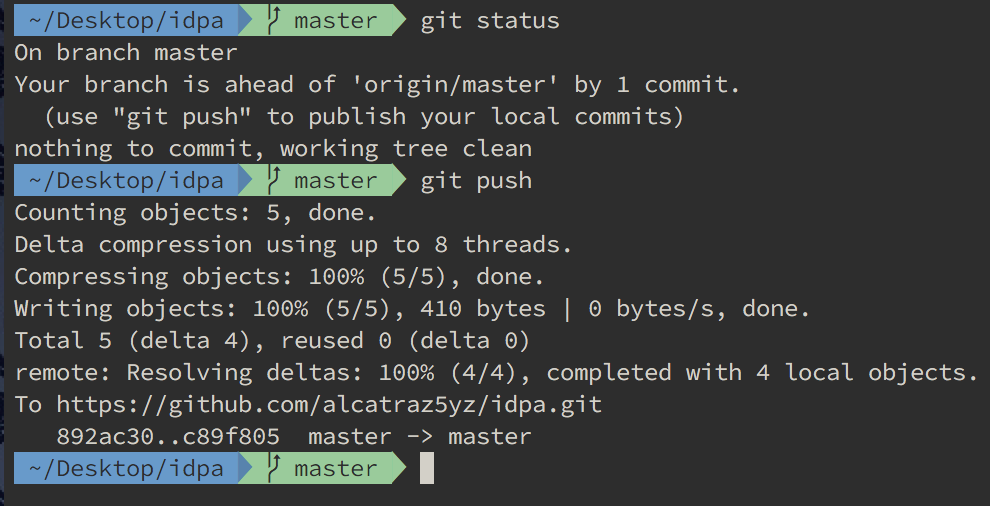
\includegraphics[width=.8\linewidth]{cli-git}
            \caption{Beispiel Termin}
            \label{fig:sub1}{Hier schiebe ich mein lokales Git Repository
            hinauf zu Github.
            d.h. ich speichere mein Ordner auf Github}
            \end{figure}

            \begin{figure}[ht]
                \centering
                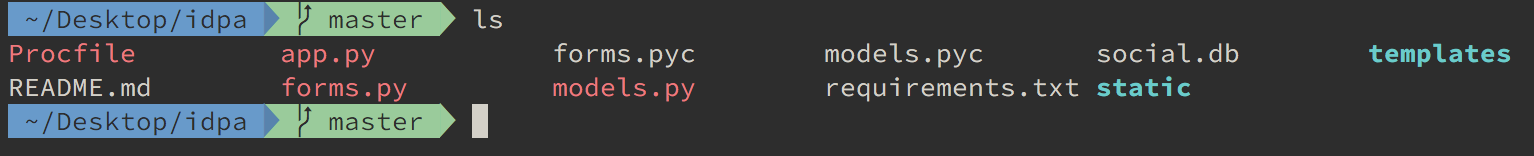
\includegraphics[width=.9\linewidth]{cli-ls}
                \caption{Beispiel Termin}
                \label{fig:sub1}{wenn man ls im terminal schreibt, kann man sehen was alles im Ordner drin ist.}
                \end{figure}


            \begin{figure}[ht]
                \centering
                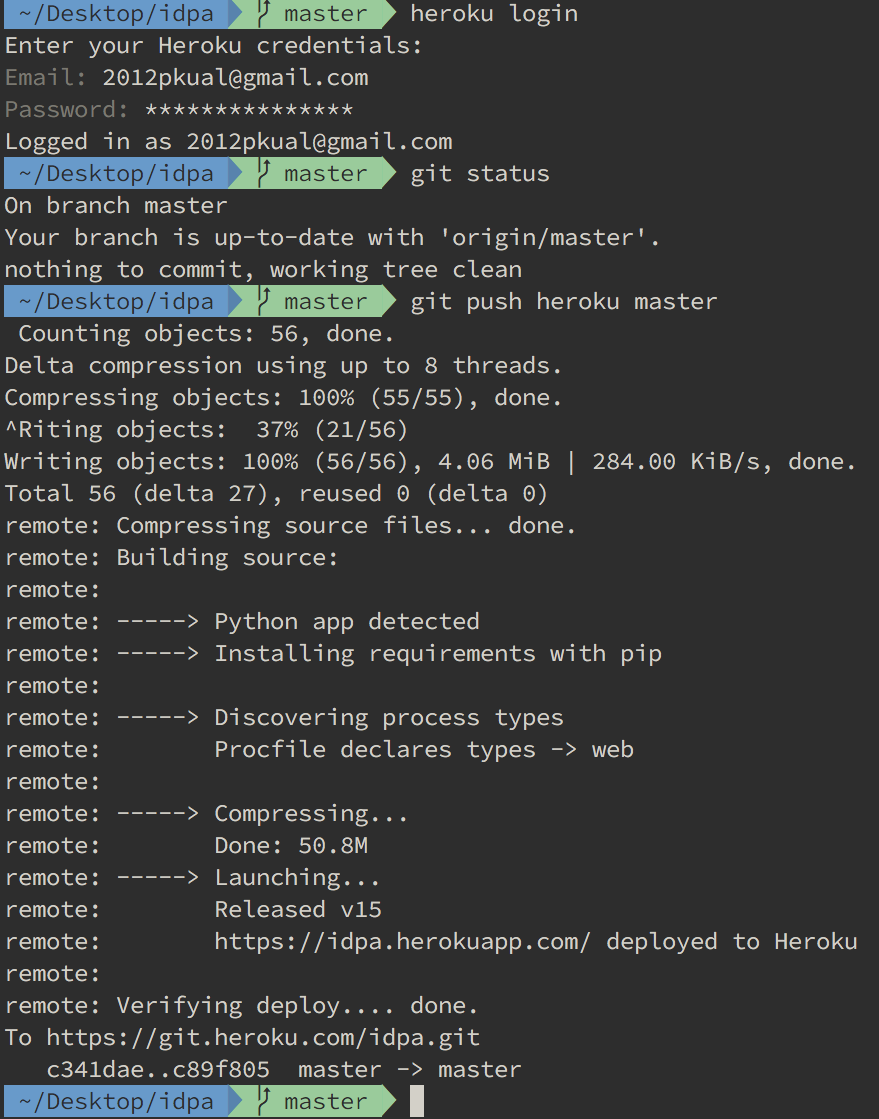
\includegraphics[width=.8\linewidth]{cli-heroku}
                \caption{Beispiel Terminal}
                \label{fig:sub1}{Hier aktualisiere ich meine Webseite welche schon Frei zug"anglich ist.
                Mit dem Terminal und Heroku geht das ganz einfach mit wenigen Commands.}
                \end{figure}
\cleardoublepage










\section{Erstellen der Seite}
Nun Zeige ich wie ich die Webseite erstellt habe, das heisst ich werde den Code pr"asentieren, und zeigen was er macht.
Es ist viel Code im Vergleich zum Game, deshalb zeige ich nur das Routing der Webseite und die Logik hinter dem Login.
Vom Javascript-code und vom Css-code und den Anderen html Seiten zeige ich auch nichts, weil das Tausende von code-Zeilen w?ren, d.h. ich w?rde die Seiten praktisch nur
mit Code f?llen und das will ich nicht. Wenn du dich daf?r interessierst,
schau sie dir einfach bei mir auf Github an.\\


\subsection{Routing}
Hier schreibe ich die Organisation von der ganzen Seite, das heisst wo was aufgerufen wird.
Dies steht im app.py file.\\
\\
Alles n?tige muss importiert werden.


\begin{lstlisting}
  from flask import (Flask, g, render_template, flash, redirect, url_for,
                abort)
from flask_bcrypt import check_password_hash
from flask_login import (LoginManager, login_user, logout_user,
                           login_required, current_user)

import forms
import models
\end{lstlisting}

der Port/Host wird festgelegt und Debug = TRUE heisst es kann jederzeit ?nderungen
vorgenommen werden.

\begin{lstlisting}
  DEBUG = True
  PORT = 8000
  HOST = '0.0.0.0'
\end{lstlisting}


kreiere loginmanager
\begin{lstlisting}
  app = Flask(__name__)
  app.secret_key = 'auoesh.bouoastuh.43,uoausoehuosth3ououea.auoub!'

  login_manager = LoginManager()
  login_manager.init_app(app)
  login_manager.login_view = 'login'

  @login_manager.user_loader
  def load_user(userid):
    try:
        return models.User.get(models.User.id == userid)
    except models.DoesNotExist:
        return None
\end{lstlisting}



Verbindung mit der Datenbank vor und nach der Nachfrage
\begin{lstlisting}
  @app.before_request
  def before_request():
    """Connect to the database before each request."""
    g.db = models.DATABASE
    g.db.connect()
    g.user = current_user


  @app.after_request
  def after_request(response):
    """Close the database connection after each request."""
    g.db.close()
    return response
\end{lstlisting}


Routing allen Seiten

\begin{lstlisting}
  @app.route('/register', methods=('GET', 'POST'))
  def register():
    form = forms.RegisterForm()
    if form.validate_on_submit():
        flash("Yay, you registered!", "success")
        models.User.create_user(
            username=form.username.data,
            email=form.email.data,
            password=form.password.data
        )
        return redirect(url_for('index'))
    return render_template('register.html', form=form)


  @app.route('/login', methods=('GET', 'POST'))
  def login():
    form = forms.LoginForm()
    if form.validate_on_submit():
        try:
            user = models.User.get(models.User.email == form.email.data)
        except models.DoesNotExist:
            flash("Your email or password doesn't match!", "error")
        else:
            if check_password_hash(user.password, form.password.data):
                login_user(user)
                flash("You've been logged in!", "success")
                return redirect(url_for('index'))
            else:
                flash("Your email or password doesn't match!", "error")
    return render_template('login.html', form=form)


  @app.route('/logout')
  @login_required
  def logout():
    logout_user()
    flash("You've been logged out! Come back soon!", "success")
    return redirect(url_for('index'))


  @app.route('/new_post', methods=('GET', 'POST'))
  @login_required
  def post():
    form = forms.PostForm()
    if form.validate_on_submit():
        models.Post.create(user=g.user.id,
                           content=form.content.data.strip())
        flash("Message posted! Thanks!", "success")
        return redirect(url_for('stream'))
    return render_template('post.html', form=form)


  @app.route('/')
  def index():
    return render_template('index.html')

  @app.route('/about')
  @login_required
  def about():
    return render_template('about.html')

  @app.route('/paint')
  @login_required
  def paint():
    return render_template('paint.html')

  @app.route('/gallery')
  @login_required
  def gallery():
    return render_template('gallery.html')

  @app.route('/game')
  @login_required
  def game():
    return render_template('game.html')


  @app.route('/game2')
  @login_required
  def game2():
    return render_template('game2.html')





  @app.route('/stream')
  @app.route('/stream/<username>')
  def stream(username=None):
    template = 'stream.html'
    if username and username != current_user.username:
        try:
            user = models.User.select().where(
                models.User.username**username).get()
        except models.DoesNotExist:
            abort(404)
        else:
            stream = user.posts.limit(100)
    else:
        stream = current_user.get_stream().limit(100)
        user = current_user
    if username:
        template = 'user_stream.html'
    return render_template(template, stream=stream, user=user)


  @app.route('/post/<int:post_id>')
  def view_post(post_id):
    posts = models.Post.select().where(models.Post.id == post_id)
    if posts.count() == 0:
        abort(404)
    return render_template('stream.html', stream=posts)


  @app.route('/follow/<username>')
  @login_required
  def follow(username):
    try:
        to_user = models.User.get(models.User.username**username)
    except models.DoesNotExist:
        abort(404)
    else:
        try:
            models.Relationship.create(
                from_user=g.user._get_current_object(),
                to_user=to_user
            )
        except models.IntegrityError:
            pass
        else:
            flash("You're now following {}!".format(to_user.username), "success")
    return redirect(url_for('stream', username=to_user.username))

  @app.route('/unfollow/<username>')
  @login_required
  def unfollow(username):
    try:
        to_user = models.User.get(models.User.username**username)
    except models.DoesNotExist:
        abort(404)
    else:
        try:
            models.Relationship.get(
                from_user=g.user._get_current_object(),
                to_user=to_user
            ).delete_instance()
        except models.IntegrityError:
            pass
        else:
            flash("You've unfollowed {}!".format(to_user.username), "success")
    return redirect(url_for('stream', username=to_user.username))
\end{lstlisting}




Der Errorhandler ist da falls die Website nicht gefunden werden kann,
dann wird direkt zur Seite 404.html weitergeleitet.
\begin{lstlisting}
  @app.errorhandler(404)
  def not_found(error):
    return render_template('404.html'), 404

\end{lstlisting}

Initialisierung

\begin{lstlisting}
  if __name__ == '__main__':
    models.initialize()
    try:
        models.User.create_user(
            username='allan',
            email='2012pkual@gmail.com',
            password='password',
            admin=True
        )
    except ValueError:
        pass
    app.run(debug=DEBUG, host=HOST, port=PORT)
\end{lstlisting}



\end{lstlisting}














\cleardoublepage
\subsection{Login}

Nun kommt die Organisation f"ur das Login, welches in forms.py steht

\begin{figure}[ht]
    \centering
    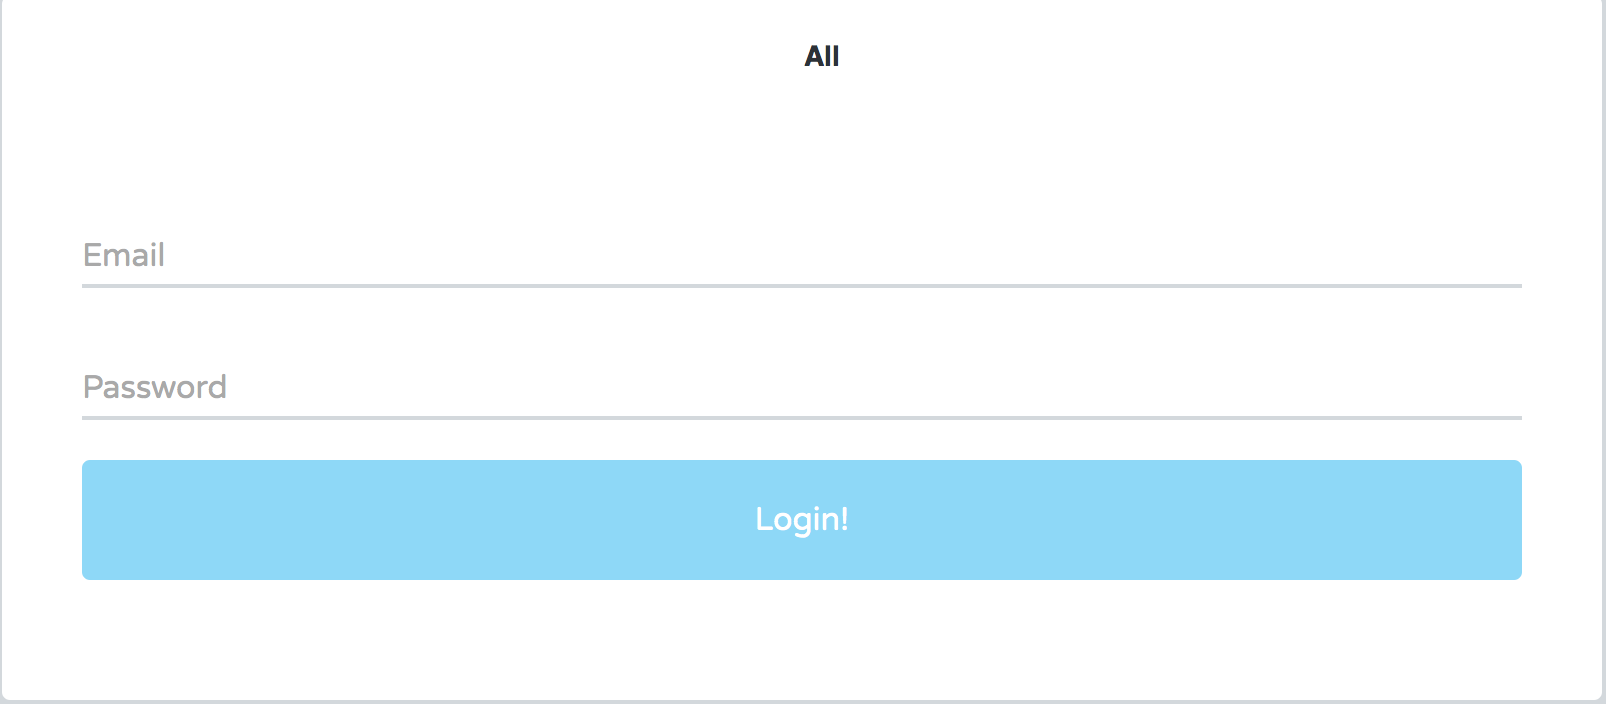
\includegraphics[width=1\linewidth]{login}
    \caption{Login}
    \label{fig:sub1}
    \end{figure}\\

\\
Notwendige Importe
\begin{lstlisting}
  from flask_wtf import Form
  from wtforms import StringField, PasswordField, TextAreaField
  from wtforms.validators import (DataRequired, Regexp, ValidationError, Email,
                               Length, EqualTo)

  from models import User

\end{lstlisting}




Falls User bereits existiert.
\begin{lstlisting}
  def name_exists(form, field):
      if User.select().where(User.username == field.data).exists():
          raise ValidationError('User with that name already exists.')


  def email_exists(form, field):
      if User.select().where(User.email == field.data).exists():
          raise ValidationError('User with that email already exists.')
\end{lstlisting}





Registrierungsform wird deklariert.

\begin{lstlisting}
  class RegisterForm(Form):
      username = StringField(
          'Username',
          validators=[
              DataRequired(),
              Regexp(
                  r'^[a-zA-Z0-9_]+',
                  message=("Username should be one word, letters, "
                           "numbers, and underscores only.")
              ),
              name_exists
          ])
\end{lstlisting}






Bedingungen werden erstellt z.B: dass man das Passwort zweimal eingeben muss
bei der Registrierung.
\begin{lstlisting}
  email = StringField(
      'Email',
      validators=[
          DataRequired(),
          Email(),
          email_exists
      ])
  password = PasswordField(
      'Password',
      validators=[
          DataRequired(),
          Length(min=2),
          EqualTo('password2', message='Passwords must match')
      ])
  password2 = PasswordField(
      'Confirm Password',
      validators=[DataRequired()]
  )

\end{lstlisting}





LoginForm schaut nach ob Daten ?bereinstimmen
\begin{lstlisting}
  class LoginForm(Form):
      email = StringField('Email', validators=[DataRequired(), Email()])
      password = PasswordField('Password', validators=[DataRequired()])


  class PostForm(Form):
      content = TextAreaField("What's up?", validators=[DataRequired()])
\end{lstlisting}


















\cleardoublepage


























































\section{Game}
Mein Game werde ich nun gleich pr"asentieren wie die Webseite,das heisst ich werde wieder zeigen was der Code macht und welche bilder ich ben"otigt habe.
\begin{figure}[ht]
    \centering
    
\includegraphics[width=.5\linewidth]{phaser}
    \caption{Phaser-Logo}
    \label{fig:sub1}
    \end{figure}


    \subsection{Sounds}
    Ich habe 4 verschiedene Arten von Sound ins Game eingebaut.\\
    Ein Sound ist das Ganze Spiel ?ber aktiv und ist sowas wie die Hintergrundmusik des Games.\\
    Der Zweite Sound wird abgespielt wenn entweder das Gameover oder youWin oder Play im Startmenu ausgew"ahlt wird.\\
    Der Dritte Sound ist ein Schmerz-Sound der abgespielt wird wenn der Spieler getroffen wird.\\
    Der vierte Sound ist derjenige f"ur die Waffe des Spielers, sie wird aktiviert, wenn einer der Meteoriten abgeschossen wird.\\




\subsection{Meine Verwendeten Bilder und Sprites}
Bei Bilder welche z.B. laufen sollen im Game, bei denen kann ich nicht nur ein Bild einsetzen, sondern ich brauche ein Spritesheet,
d.h. ein Bild von jeder Bewegung im Raum.
Denn wenn der Player nach rechts geht, will man ja die Seite des Spielers sehen und nicht seine Vorderseite.



\begin{figure}[ht]
\centering
\begin{subfigure}{.5\textwidth}
  \centering
  
\includegraphics[width=.3\linewidth]{diamond}
  \caption{Diamant}
  \label{fig:sub1}
\end{subfigure}%
\begin{subfigure}{.5\textwidth}
  \centering
  
\includegraphics[width=.6\linewidth]{dude}
  \caption{Player}
  \label{fig:sub2}
\end{subfigure}
% \caption{}
% \label{fig:test}
% \caption[short title]{}
\end{figure}


\begin{figure}[ht]
\centering
\begin{subfigure}{.5\textwidth}
  \centering
  
\includegraphics[width=.3\linewidth]{explosion}
  \caption{Explosion beim Klicken}
  \label{fig:sub1}
\end{subfigure}%
\begin{subfigure}{.5\textwidth}
  \centering
  \includegraphics[width=.3\linewidth]{titleBG}
  \caption{Hintergrundbild}
  \label{fig:sub2}
\end{subfigure}
% \caption{}
% \label{fig:test}
% \caption[short title]{}
\end{figure}



\begin{figure}[ht]
\centering
\begin{subfigure}{.5\textwidth}
  \centering
  
\includegraphics[width=.1\linewidth]{ghost}
  \caption{Geist wenn der Spieler getroffen wird}
  \label{fig:sub1}
\end{subfigure}%
\begin{subfigure}{.5\textwidth}
  \centering
  
\includegraphics[width=.3\linewidth]{loader_bar}
  \caption{Ladebalken}
  \label{fig:sub2}
\end{subfigure}
% \caption{}
% \label{fig:test}
% \caption[short title]{}
\end{figure}




\begin{figure}[ht]
\centering
\begin{subfigure}{.5\textwidth}
  \centering
  
\includegraphics[width=.3\linewidth]{platform}
  \caption{Die Platform wo der Player sich drauf herumbewegt}
  \label{fig:sub1}
\end{subfigure}%
\begin{subfigure}{.5\textwidth}
  \centering
  
\includegraphics[width=.3\linewidth]{sky}
  \caption{Hintergrundbild beim Hauptgame}
  \label{fig:sub2}
\end{subfigure}
% \caption{}
% \label{fig:test}
% \caption[short title]{}
\end{figure}




\begin{figure}[ht]
\centering
\begin{subfigure}{.5\textwidth}
  \centering
  \includegraphics[width=.3\linewidth]{spacerock}
  \caption{Meteorit}
  \label{fig:sub1}
\end{subfigure}%
\begin{subfigure}{.5\textwidth}
  \centering
  
\includegraphics[width=.3\linewidth]{star}
  \caption{Stern}
  \label{fig:sub2}
\end{subfigure}
% \caption{}
% \label{fig:test}
% \caption[short title]{}
\end{figure}








\cleardoublepage





\subsection{Game Teil1: index.html}

Im index.html file sind die Referenzen zu den anderen 4
js-files boot/Preloader/StartMenu/Game, als auch der Verweis zum Phaser js-file

\begin{lstlisting}
  <script src="libs/phaser.js"></script>
  <script src="Boot.js"></script>
  <script src="Preloader.js"></script>
  <script src="StartMenu.js"></script>
  <script src="Game.js"></script>
\end{lstlisting}


index.html beinhaltet keine Funktionen welche f"ur das Game von Bedeutung w"aren, das heisst der Inhalt des Games wird in den 4 Js-files erstellt.
im index.html file wird nur alles zusammengef"uhrt und dann ausgef"uhrt weil es ja ein html file ist.
Der Link zum Phaser Hauptfile phaser.js ist auch hier eingebunden.
am Schluss vom FIle wird das File Boot.js aufgerufen



\begin{lstlisting}
    game.state.start('Boot');
\end{lstlisting}



\subsection{Game Teil2: Boot.js}

Im Boot.js werden die Grundlagen f"ur das Game erstellt.

\begin{lstlisting}
  create: function() {
        this.input.maxPointers = 1; //nur ein curser
        this.stage.disableVisibilityChange = false; //pauses the game when open another tab
        this.scale.scaleMode = Phaser.ScaleManager.SHOW_ALL;
        this.scale.minWidth = 270;
        this.scale.minHeight = 480;
        this.scale.pageAlignHorizontally = true;//center game
        this.scale.pageAlignVertically = true;//center game
        this.stage.forcePortrait = true;
        this.scale.setScreenSize(true);//force ScreenSize
        this.input.addPointer();
        this.stage.backgroundColor = '#171642';

        this.state.start('Preloader');
    }
\end{lstlisting}

Hier sieht man, dass ich maximal 1 curser habe.\\
Das Game wird gestoppt, wenn ich die Seite verlasse, d.h. ein anderer Tab "offne oder das Fenster wechsle.\\
Es wird das Gesamtbild organisiert.\\
Die Hintergrundfarbe des Games ist #171642 was dunkelblau ist.\\
Am Schluss wird das File Preloader.js aufgerufen.\\



\cleardoublepage
\subsection{Game Teil3: Preloader.js}



Mein Game besteht aus drei Fenstern sozusagen, dem Ladefenster, dem Startmenufenster und dem Game selber.?\\
Hier im Preloader.js wird das Ladefenster kreiert, welches aus Hintergrundbild und Ladebalken besteht.\\
diese Zwei Bilder wurden im vorherigen File Boot.js geladen.\\

\begin{lstlisting}
  Survive.Boot.prototype = {
      preload: function() {
          this.load.image('preloaderBar', 'images/loader_bar.png');
      },
\end{lstlisting}

Hier oben wird der Ladebalken geladen

\begin{lstlisting}
  Survive.Boot.prototype = {
  create: function() {
this.stage.backgroundColor = '#171642';
}
}
\end{lstlisting}
Hier oben wird das Hintergrundbild geladen.\\
Im Preloader.js File werden alle Bilder und Sounds welche f?r das Startmenu und das Game sind geladen.


\begin{lstlisting}
          Survive.Preloader.prototype = {
          preload: function () {
          this.load.image('titlescreen', 'images/TitleBG.png');
          this.load.bitmapFont('eightbitwonder', 'fonts/eightbitwonder.png', 'fonts/eightbitwonder.fnt');
          this.load.image('sky', 'images/sky.png');
          this.load.atlasXML('spacerock', 'images/spritesheets/SpaceRock.png', 'images/spritesheets/SpaceRock.xml');
          this.load.image('explosion', 'images/explosion.png');
          this.load.image('platform', 'images/platform.png');
          this.load.image('diamond', 'images/diamond.png');
          this.load.image('star', 'images/star.png');
          this.load.spritesheet('dude', 'images/dude.png', 32, 48);
          this.load.image('ghost', 'images/ghost.png');
          this.load.audio('explosion_audio', 'audio/explosion.mp3');
          this.load.audio('hurt_audio', 'audio/hurt.mp3');
          this.load.audio('select_audio', 'audio/select.mp3');
          this.load.audio('game_audio', 'audio/bgm.mp3');
      },
\end{lstlisting}


Die Animation f"ur den Ladebalken:
\begin{lstlisting}
  preload: function () {
        this.preloadBar = this.add.sprite(this.world.centerX, this.world.centerY, 'preloaderBar');
        this.preloadBar.anchor.setTo(0.5, 0.5);
        this.load.setPreloadSprite(this.preloadBar);
        }
\end{lstlisting}

An Schluss wird das File Startmenu.js aufgerufen.\\


\begin{lstlisting}
    game.state.start('StartMenu');
\end{lstlisting}

\cleardoublepage
\subsection{Game Teil4: Startmenu.js}

Im Starmenu erstelle ich das zweite Bild, n?mlich dieses:

\begin{figure}[ht]
    \centering
    
\includegraphics[width=.3\linewidth]{foto}
    \caption{Startmenu}
    \label{fig:sub1}{Dies sieht man beim Starmenu}
    \end{figure}

Zuerst kreiere ich das Bild mit dem Text'Press to Start' drauf
\begin{lstlisting}
  image = this.add.image(0, 0, 'titlescreen');
    text = this.add.bitmapText(this.world.centerX-155,
    this.world.centerY+280, 'eightbitwonder', 'Press to Start', 24);
        text.inputEnabled = true;
        text.events.onInputDown.addOnce(this.startGame, this);
\end{lstlisting}

Wenn ich das Bild anklicke, sollte es ja ein ger"ausch machen, um mir zu signalisieren, dass es funktioniert hat.
Deshalb baue ich noch das Ger"ausch ein.

\begin{lstlisting}
this.audio = this.add.audio('select_audio');
this.audio.play();
\end{lstlisting}
Da ja alles schon geladen ist, muss ich nur es noch einsetzen.\\
Am Schluss wird das File Startmenu.js aufgerufen.\\

\begin{lstlisting}
    game.state.start('Game');
\end{lstlisting}

\cleardoublepage
\subsection{Game Teil5: Game.js}


Am Schluss kreiere ich das dritte Fenster, n"amlich das Game.
hier ein Ausschnitt:

\begin{figure}[ht]
    \centering
    \includegraphics[width=.5\linewidth]{dude1}
    \caption{Bild vom Game}
    \label{fig:sub1}{Hier sieht man wie alles zusammengef?gt aussieht.}
    \end{figure}


Im Game hat es viele Sachen und Aktionen welche kreiert werden m"ussen.
Zuerst kommen wieder die Grundbedingungen:

\begin{lstlisting}
  create: function() {
        this.cursors = this.input.keyboard.createCursorKeys();
        this.ouch = this.add.audio('hurt_audio');
        this.boom = this.add.audio('explosion_audio');
        this.ding = this.add.audio('select_audio');
        this.music = this.add.audio('game_audio');
        this.music.play('', 0, 0.3, true);
        this.gameover = false;
        this.totalStars = 1;
        this.totalSpacerocks = 200;
        this.physics.startSystem(Phaser.Physics.ARCADE);
        this.buildWorld();
    },
\end{lstlisting}


Ich beginne dann St"uck f"ur St"uck die Einzelnen Teile hinzuzuf"ugen.
Ich beginne mit dem Boden und den Ebenen in der Luft:
Zus"atzlich noch das Hintergrundbild (sky)

\begin{lstlisting}
  buildWorld: function() {
      this.add.sprite(0, 0, 'sky');
      platforms = this.add.group();
      platforms.enableBody = true;
       this.ground = platforms.create (0, this.world.height - 64, 'platform');
      this.ground.scale.setTo(2, 2);
      this.ground.body.immovable = true;
      this.ledge = platforms.create(350, 150, 'platform');
      this.ledge.body.immovable = true;
      this.ledge = platforms.create(-150, 290, 'platform');
      this.ledge.body.immovable = true;
      this.ledge = platforms.create(350, 490, 'platform');
      this.ledge.body.immovable = true;
      this.ledge = platforms.create(-150, 650, 'platform');
      this.ledge.body.immovable = true;
      this.ledge = platforms.create(350, 750, 'platform');
      this.ledge.body.immovable = true;
\end{lstlisting}

So wird der Spieler kreiert:

\begin{lstlisting}
  this.player = this.add.sprite(32, this.world.height - 150, 'dude');
          this.physics.arcade.enable(this.player);
          this.player.body.bounce.y = 0.2;
          this.player.body.gravity.y = 300;
          this.player.body.collideWorldBounds = true;
          this.player.animations.add('left', [0, 1, 2, 3], 10, true);
          this.player.animations.add('right', [5, 6, 7, 8], 10, true);
\end{lstlisting}


Die Sterne:


\begin{lstlisting}
  this.stars = this.add.group();
      this.stars.enableBody = true;
      for (var i=0; i<this.totalStars; i++)
          {
      star = this.stars.create(i * 70, 0, 'star');
      star.body.gravity.y = 300;
      star.body.bounce.y = 0.7 + Math.random() * 0.2;
          }
\end{lstlisting}

die Meteoriten:

\begin{lstlisting}
this.buildSpaceRocks();
buildSpaceRocks: function() {
        this.spacerockgroup = this.game.add.group();
        for(var i=0; i<this.totalSpacerocks; i++) {
            var rock = this.spacerockgroup.create(this.rnd.integerInRange(0,
            this.world.width),
            this.rnd.realInRange(-1500, 0), 'spacerock', 'SpaceRock0000');
            var scale = this.rnd.realInRange(0.3, 1.0);
            rock.scale.x = scale;
            rock.scale.y = scale;
            this.physics.enable(rock, Phaser.Physics.ARCADE);
            rock.enableBody = true;
            rock.body.velocity.y = this.rnd.integerInRange(200, 400);
            rock.animations.add('Fall');
            rock.animations.play('Fall', 24, true);
            rock.checkWorldBounds = true;
            rock.events.onOutOfBounds.add(this.resetRock, this);
            this.physics.arcade.overlap(this.player, rock,
            this.playerCollision, null, this);

        }
    },


    resetRock: function(rock) {
        if(rock.y > this.world.height) {
            this.respawnRock(rock);
        }
    },

    respawnRock: function(rock) {
        if(this.gameover == false){
            rock.reset(this.rnd.integerInRange(0, this.world.width),
            this.rnd.realInRange(-1500, 0));
            rock.body.velocity.y = this.rnd.integerInRange(200, 400);
        }
    },

\end{lstlisting}

die Explosionen beim Tippen:
\begin{lstlisting}
    this.buildEmitter();
    buildEmitter:function() {
        this.burst = this.add.emitter(0, 0, 80);
        this.burst.minParticleScale = 0.3;
        this.burst.maxParticleScale = 1.2;
        this.burst.minParticleSpeed.setTo(-30, 30);
        this.burst.maxParticleSpeed.setTo(30, -30);
        this.burst.makeParticles('explosion');
        this.input.onDown.add(this.fireBurst, this);
    },

    fireBurst: function(pointer) {
        if(this.gameover == false){
            this.boom.play();
            this.boom.volume = 0.2;
            this.burst.emitX = pointer.x;
            this.burst.emitY = pointer.y;
            this.burst.start(true, 200, null, 20);
        }
    },
\end{lstlisting}


Ich erstelle den Geist wenn der Spieler stirbt.

\begin{lstlisting}
  makeGhost: function(player) {
      playerghost = this.add.sprite(player.x-20, player.y-180, 'ghost');
      playerghost.anchor.setTo(0.5, 0.5);
      playerghost.scale.x = player.scale.x;
      this.physics.enable(playerghost, Phaser.Physics.ARCADE);
      playerghost.enableBody = true;
      playerghost.checkWorldBounds = true;
      playerghost.body.velocity.y = -800;
\end{lstlisting}


\cleardoublepage






\section{Zusammenfassung}
Zuerst wollte ich nur ein Game in Python entwickeln, aber dann merkte ich,
dass ich in der Webseiteentwicklung bereits mehr erfahrung hatte.\\
Es gibt einen grossen Unterschied zwischen einer einfachen Webseite,
welche beinahe keine grosse Komplexit"at enth"alt nur mit hmtl und css, und einer Webseite welche Komplizierter ist und auch
Backend betrieben wird, d.h. mit einer Serverside Sprache vervollst"andigt werden muss.\\
In meiner Webseite habe ich dies mit Python-Flask verwirklicht und auch noch eine
Datenbank mit eingebracht, welche Speichert, wenn sich eine neue Person bei meiner
Webseite einschreibt.\\
Ich brauchte auch noch Kenntnisse beim ben"utzen des Terminals,Github,Git und virtualenv, um
alles machen zu k?nnen.\\
Bei der Zwischen-Pr"asentation sagten mir die Lehrer dann aber,
dass es noch nicht reichen w"urde, deshalb musste ich noch ein Spiel einbringen.\\
Nat"urlich musste es ein Spiel sein, welches ich in die Webseite einsetzen konnte.\\
Ich wusste, dass es bereits Spiele f"ur das Web genannt htmlt5-games gab und wusste
auch schon wo zu suchen und so kam ich zur Gameengine phaser.\\
Nun zum Schluss habe ich eine Webseite mit Games, Blog, und Login kreiert
und sie auch mithilfe von Heroku hochgeladen damit sie jeder anschauen kann.\\
Dieses Dokument habe ich mit Latex geschrieben um vor allem meine Kenntnisse darin zu
verbessern, denn eigentlich ist es aufw"andiger ein Latex-File zu programmieren als das Dokument
einfach mit Microsoft Word zu schreiben.\\
Von der Zeit her hatte ich schnell stress, denn es lief selten wie geplant.\\
Oftmals funktionierte etwas nicht, weil ich einen Fehler machte oder sonst etwas vergessen habe.\\
Wenn es Fehler gab musste ich oft Stunden oder sogar Tage daf"ur investieren ihn zu finden und zu l"osen.\\
Obwohl es viele Probleme gab, hat es mir sehr gefallen zu programmieren.


\cleardoublepage

\section{Summary}
First I just wanted to develop a game made in Python but then I realized,
that I've had already more experience in webdevelopment.\\
There is a big difference between creating just a simple website, which has almost no komplexity built in,
with just plain html and css and a website who is more komplex and also works on the Backend, which means you have to complete it with a
serverside language.\\
In my website I have realised this with Python-Flask plus I have also put in a database, who stores the data, if a new Person wants to Sign-in
on my website.\\
to create all this, I also needed more knowledge on using the Terminal,Github,Git and virtualenv.\\
During the middle-presentation, my teachers told that this wasn't enough, so I had to put in game.\\
Of course it had to be a game, which I could add to the website.\\
I knew already that there were games for the web called html5-games and I already knew where to look, so I ended up with the game-engine called phaser.\\
At the end I have created a website with games, blog and a login plus I deployed it successfully to heroku, so that everyone can watch it.\\
I have created this Document with the Language Latex for the sole purpose of strengthening my knowledge in it, because it requires actually more effort
to create the textfile than doing it with Microsoft Word.\\
It was stressing all the time, because my programms rarely worked as planned.\\
Often it didn't work because I have made a mistake or I have forgotten something.\\
If there was a mistake, I had to search for hours or even days to find it and solve it.\\
Even if there were a lot of problems, I enjoyed programming it.\\

\cleardoublepage




\section{Literaturverzeichnis}
\subsection{B"ucher}

Oetiker Tobias: The Not So Short Introduction to LATEX 2E OR lATEX in 157 minutes,version 5.05,July 18, 2015\\
                LATEX for Beginners. Workbook, Edition 5, M?rz 2014 Document-Referenz 3722-2014\\
Jorge Palacios:Developing an HTML5 BRICK-BREAKER game with PHASER. Band1, Leanpub, Ort, 2015-05-31\\
Geoffrey M.Poore:The pythontex package. Band1, LPPL,\\





\subsection{Webseiten}

phaser:https://phaser.io/\\
flask:http://flask.pocoo.org/\\
texteditors:\\
 atom:https://atom.io/\\
 brackets:http://brackets.io/\\
 sublime text 3:https://www.sublimetext.com/\\
jqueryrain:http://www.jqueryrain.com/\\
Css :https://www.mediaevent.de/css/\\
Git/version control:https://git-scm.com/\\
Github :https://github.com/\\
heroku :https://www.heroku.com/\\
teamtreehouse :https://www.overleaf.com/\\
lynda: https://www.overleaf.com/\\
codacademy :https://www.overleaf.com/\\
Overleaf:https://www.overleaf.com/\\










\cleardoublepage




% Appendix starts here
\appendix
\section{Anhang}
Hier sind noch alle Seiten mit denen ich in ber"uhrung gekommen bin w"ahrend dem
Bearbeiten dieses Projectes\\


phaser unter https://phaser.io/\\
flask unter http://flask.pocoo.org/\\
texteditors:\\
 atom unter https://atom.io/ und schau dir das video dazu an.\\
 brackets unter http://brackets.io/\\
 sublime text 3 unter https://www.sublimetext.com/\\
wenn sublime text, dann mit package control unter https://packagecontrol.io/\\
jquery-plugins auf jqueryrain unter http://www.jqueryrain.com/\\
Css unter https://www.mediaevent.de/css/\\
Git/version control unter https://git-scm.com/\\
Github unter https://github.com/\\
heroku unter https://www.heroku.com/\\
teamtreehouse unter https://www.overleaf.com/\\
lynda unter https://www.overleaf.com/\\
codacademy unter https://www.overleaf.com/\\
latex auf Overleaf unter https://www.overleaf.com/\\
\\
Schau dir doch noch mein Zeugs an.\\
meine Webseite auf Heroku unter http://idpa.herokuapp.com\\
mein Code der Webseite auf Github unter https://github.com/alcatraz5yz/idpa\\





\end{document}
